\chapter{Minimum Entropy Coupling with Bottleneck}\label{ch:mecb}

\section{Introduction}\label{ch3:sec:introduction}

Consider the following Markov Chain modeling a general lossy compression framework:

\begin{equation}
    X \xrightarrow{\enc_{T|X}} T \xrightarrow{\dec_{Y|T}} Y
\end{equation}

Here, the input $X$, with a marginal distribution $p_X$, is encoded by the probabilistic encoder \enc to generate the code $T$. Subsequently, the probabilistic decoder \dec constructs $Y$ from $T$. The objective is to identify the encoder and decoder that minimize the distortion between $X$ and $Y$, subject to a constraint on the expected code length $H(T)$.

It is common to measure the sample-wise distortion via direct comparison of $(x, y)$ pairs through a distortion function $d(\cdot, \cdot)$, and consider the expectation $\ex \left[ d(X,Y)  \right]$ as a measure of average distortion. Instead, we propose using the logarithmic loss (log-loss) $H(X|Y)$, or equivalently $I(X;Y)$, as an alternative metric to enforce the distortion constraint.

The log-loss distortion measure, commonly employed in learning theory, was first explored within rate-distortion theory by \cite{courtade2011multiterminal} and \cite{courtade2013multiterminal}. This measure is particularly suitable in scenarios where reconstructions can be soft, meaning that the decoder produces a distribution rather than a distorted sample point \cite{shkel2017single}. Consequently, the optimization problem is formulated as follows:

\begin{equation}
\begin{aligned} \label{ch3:eq:no_const}
    &\min_{\enc_{T|X},\; \dec_{Y|T}} \hspace{-1em} &&H(X|Y) \\
    &\hspace{2em} \textrm{s.t.} &&X \leftrightarrow T \leftrightarrow Y, \\
    & &&H(T) \leq R, \\
    & &&P(X) = p_X
\end{aligned}
\end{equation}

It is straightforward to check that the optimal solution of (\ref{ch3:eq:no_const}) is achieved when $T=Y$, with the identity decoder. To address this issue of decoder collapse, we introduce a constraint on the output marginal distribution, $P(Y)$:

\eqtcb{Minimum Entropy Coupling with Bottleneck (MEC-B)}{
\begin{equation}
% \tag{MEC-B}
\begin{aligned}\label{ch3:eq:mecb}
    \MECB(p_X, p_Y, R) = &\max_{\enc_{T|X},\; \dec_{Y|T}} \hspace{-1em} &&I(X;Y) \\
    &\hspace{2em} \textrm{s.t.} &&X \leftrightarrow T \leftrightarrow Y, \\
    & &&H(T) \leq R, \\
    & &&P(Y) = p_Y, \\
    & &&P(X) = p_X
\end{aligned}
\end{equation}
}

We explore two special cases of \eqref{ch3:eq:mecb}, where either the encoder or decoder is bypassed. This allows us to optimize the encoder and decoder separately using these cases.

First, consider the case where the bottleneck is removed, meaning the constraint $H(T) \leq R$ is relaxed, or $R \geq H(X)$. In this scenario, $X=T$, and the optimization simplifies to:

\eqtcb{Minimum Entropy Coupling (MEC)}{
\begin{equation} 
% \tag{MEC}
\begin{aligned} \label{ch3:eq:mec}
    \MEC(p_X, p_Y) = \max_{\enc_{Y|X}} \ &I(X;Y) \\
    \textrm{s.t.} \ \ &P(Y) = p_Y, \\
    &P(X) = p_X
\end{aligned}
\end{equation}
}

This involves identifying the probabilistic coupling $p_{Y|X}$ between the marginals $p_X$ and $p_Y$ that maximizes the obtained mutual information. 
This problem, as described in \eqref{ch3:eq:mec}, has been extensively studied in the literature as minimum entropy coupling (MEC), with early research conducted by \cite{vidyasagar2012metric, painsky2013memoryless, kovavcevic2015entropy, cicalese2017find}, among others.
Thus, we define the original problem presented in \eqref{ch3:eq:mecb} as minimum entropy coupling with bottleneck (MEC-B).

Next, consider the case where the decoder is removed, resulting from the relaxation of the output distribution constraint in \eqref{ch3:eq:mecb}:

\eqtcb{Entropy-Bounded Information Maximization (EBIM)}{
\begin{equation}
% \tag{EBIM}
\begin{aligned}\label{ch3:eq:comp}
    \COMP(p_X, R) = &\max_{\enc_{T|X}} &&I(X;T) \\
    & \ \textrm{s.t.} &&H(T) \leq R, \\
    & &&P(X) = p_X
\end{aligned}
\end{equation}
}

Similar to minimum entropy coupling, this problem identifies the joint distribution between two random variables that maximizes their mutual information. However, rather than imposing a marginal distribution constraint, it enforces a more flexible entropy constraint on one of the variables.


Lemma~\ref{ch3:lemma:decomp} provides a decomposition for the mutual information between input and output $I(X;Y)$, given the Markov chain $X \leftrightarrow T \leftrightarrow Y$.
 
\begin{lemma} \label{ch3:lemma:decomp}
    Given a Markov chain $X \leftrightarrow T \leftrightarrow Y$:
    \begin{equation}\label{ch3:eq:Idecomp}
        I(X;Y) = I(X;T) + I(Y;T) - I(T; X,Y)
    \end{equation}
\end{lemma}
\begin{proof}
By multiple applications of the chain rule for mutual information, i.e.,  $I(A;B,C)=I(A;B)+I(A;C|B)$, we have:
\begin{align}
    I(X;Y) &= I(X;Y,T) - I(X;T|Y) \\
    &= [I(X; T) + I(X; Y | T) ] - [ - I(T; Y) + I(T; X, Y) ] \\
    &= I(X;T) + I(Y;T) - I(T; X,Y)
\end{align}
Note that from the Markov chain property, we have $I(X; Y | T)=0$.
\end{proof}

The following lower bound on the MEC-B objective is attainable based on Lemma~\ref{ch3:lemma:decomp}:
\begin{equation}\label{ch3:eq:mecblb}
    I(X;Y) \geq I(X;T) + I(Y;T) - R
\end{equation}

In this work, we consider maximizing the lower bound \eqref{ch3:eq:mecblb} as a proxy to the main objective.
This allows a decomposition of the encoder and decoder for the MEC-B formulation in \eqref{ch3:eq:mecb}:

\begin{enumerate}
    \item \textbf{Encoder Optimization:}
    The encoder is first optimized separately, according to Entropy-Bounded Information Maximization in \eqref{ch3:eq:comp}, $\COMP(p_X, R)$, resulting in the marginal distribution $\hat{p}_T$ on the code $T$.

    \item \textbf{Decoder Optimization:}
    The decoder is then optimized by solving a minimum entropy coupling in \eqref{ch3:eq:mec} between the code and output marginals, $\MEC(\hat{p}_T, p_Y)$.
\end{enumerate}

Therefore, in terms of problems \eqref{ch3:eq:mecb}, \eqref{ch3:eq:mec}, and \eqref{ch3:eq:comp}:
\begin{align}
    \MECB(p_X, p_Y, R) &= \max_{\enc_{T|X},\ \dec_{Y|T}} \ I(X;Y) \\
    &\geq \max_{\enc_{T|X},\ \dec_{Y|T}} \ \left[ I(X;T) + I(Y;T) - R \right] \\
    % &\geq \ \max_{\enc_{T|X}} \left[I(X;T)\right] + \max_{\dec_{Y|T}} \left[I(Y;T)\right] - R \\
    &\geq \COMP(p_X, R) + \MEC(\hat{p}_T, p_Y) - R
\end{align}

Section~\ref{ch3:sec:MEC} provides an overview of the minimum entropy coupling problem. Following that, Section~\ref{ch3:sec:COMP} focuses on the entropy-bounded information maximization problem as formulated in \eqref{ch3:eq:comp}, in great detail. Section~\ref{ch3:sec:mcg} discusses the application of minimum entropy coupling with bottleneck in the context of Markov Coding Games. Lastly, Section~\ref{ch3:sec:exp} presents experimental results.


% \clearpage
\section{Related Works}\label{ch3:sec:relatedworks}
\subsection{Couplings and Minimum Entropy Coupling}
A fundamental problem in probability theory, known as coupling, concerns determining the \textit{optimal} joint distribution of random variables given their marginal distributions. This problem has a long history, with early examples like \cite{frechet1951tableaux} seeking the joint distribution that maximizes correlation subject to marginal constraints. References \cite{den2012probability, lin2014recent, benes2012distributions, yu2018asymptotic} provide a broader treatment of these problem classes and their applications. Notably, optimal transport (OT) emerges as a significant class within this framework, where optimality is defined as minimizing the expected value of a loss function over the joint distribution. See \cite{villani2009optimal} for an in-depth treatment of the optimal transport problem.

The minimum entropy coupling (MEC) focuses on finding the joint distribution with the smallest entropy given the marginal distribution of some random variables. This problem has been first studied in \cite{vidyasagar2012metric, painsky2013memoryless, kovavcevic2015entropy, cicalese2017find}, among others. 
Although couplings are directly relevant to optimal transport, MEC cannot directly be framed as an optimal transport problem because the cost function in OT does not depend on the joint distribution itself. Nonetheless, given that the set of all couplings is called the transport polytope, the minimum entropy coupling is identified as the element with the lowest entropy within this transport polytope.

Entropic Optimal Transport (EOT) introduces an entropy regularization to the classical optimal transportation problem, encouraging a transport plan with high entropy. This regularization transforms the problem into a strictly convex one, eliminating the need for linear programming \cite{cuturi2013sinkhorn}. It can be efficiently solved using the Sinkhorn-Knopp matrix scaling algorithm \cite{knight2008sinkhorn}, which converges linearly and is highly parallelizable, making it exceptionally well-suited for large-scale implementations on GPUs. Note that EOT encourages couplings that exhibit high entropy, which is technically distinct from MEC, which aims for couplings with minimal entropy.

While it is shown in \cite{vidyasagar2012metric, kovavcevic2015entropy} that MEC is NP-Hard, the literature contains many approximation algorithms for this problem. One of the earliest greedy algorithms for MEC was introduced by \cite{kocaoglu2017entropic} in the context of causal inference. Specifically, the authors considered the problem of identifying the causal direction between two discrete random variables $X$ and $Y$. Generally, $X$ causes $Y$ if there exists an exogenous random variable $E$ (independent of $X$) and a deterministic function $f$ such that $Y = f (X,E)$, with the central assumption that the exogenous variable has low entropy in the true direction and high entropy in the wrong direction. They show that the problem of finding the exogenous variable with minimum entropy is equivalent to the problem of finding minimum joint entropy given marginal distributions. They propose a greedy algorithm for MEC that finds a local minimum having $1 + \log n$ bits gap from the global optimum, with $n$ being the cardinality of the support of random variables. Later in \cite{compton2022tighter}, this gap was shown to be tighter; within $\log_2(e)$ bits of the optimal.

Based on tools from the theory of majorization \cite{marshall1979inequalities}, the authors of \cite{cicalese2019minimum} developed a new greedy algorithm and demonstrated that it produces a joint distribution whose entropy exceeds the minimum possible by no more than 1 bit. They also expanded this algorithm to accommodate $k$ random variables, ensuring an additive gap of no more than $\log k$ bits. Subsequent improvements in \cite{li2021efficient} enabled the construction of a coupling whose entropy is within 2 bits of the optimal value, regardless of the number of random variables involved.

While \cite{compton2022tighter} showed that improvements beyond the majorization lower bounds are impossible, thus establishing the \textit{majorization barrier}, \cite{compton2023minimum} deviated from the majorization strategy by introducing a new technique for lower bounding the coupling entropy, termed the profile method. This approach yields stronger bounds for coupling two or more random variables.

Minimum entropy coupling finds innovative applications beyond causal inference \cite{kocaoglu2017entropic, compton2020entropic, javidian2021quantum}. For instance, \cite{sokota2022communicating} utilized it in Markov coding games to enable reinforcement learning agents to communicate via Markov decision process trajectories. This application showcased MEC's utility in enabling efficient information transmission through constrained environments like video game interactions. Similarly, \cite{de2022perfectly} applied MEC in communication but in the context of steganography, to securely encode secret information in regular text, showing MEC corresponds to the maximally efficient secure procedure.

These applications, along with those in dimension reduction of probability distribution \cite{cicalese2016approximating} and stochastic processes \cite{vidyasagar2012metric}, underline the broad applicability and significance of minimum entropy coupling across different domains of computer science and information theory.


\subsection{Information Bottlneck}
The Information Bottleneck (IB) method \cite{tishby2000information}, addresses the problem of lossy data compression and representation. The IB principle seeks an optimal trade-off between the compression of a random variable \(X\) and the fidelity of compressed representation relative to a relevant variable \(Y\). The IB problem is formalized through the following optimization objective:

\begin{equation} \label{ch3:eq:ib}
    \min_{p(t|x)} I(X;T) - \beta I(T;Y)
\end{equation}

subject to the Markov constraint $T \leftrightarrow X \leftrightarrow Y$.
Note that \(X\) is the input variable, \(Y\) is the variable of interest with which \(X\) shares mutual information, and \(T\) represents the compressed representation of \(X\).  The term \(I(X;T)\) measures the mutual information between \(X\) and its representation \(T\), serving as a quantification of the compression level, whereas \(I(T;Y)\) quantifies the preserved relevant information about \(Y\) in the representation \(T\). The parameter \(\beta > 0\) balances the trade-off between compression and fidelity.

Solving the optimization in \eqref{ch3:eq:ib} is inherently non-trivial, often requiring iterative algorithms for its resolution. The IB framework has found extensive applications across various domains, including clustering \cite{slonim2000document}, deep learning \cite{tishby2015deep, alemi2016deep}, and quantization \cite{bhatt2021information}.

Deterministic information bottleneck \cite{strouse2017deterministic} proposes a new formulation of the information bottleneck focusing on redefining the concept of compression from minimizing mutual information \(I(X; T)\) as a communication cost between \(X\) and \(T\), towards $H(T)$ from a source coding perspective that emphasizes reducing the representational cost of \(T\). 

Inherently, the information bottleneck and our proposed framework impose relevance on the compressed code in distinct ways. The differing modeling assumptions are evident from the unique Markov chain constraints within the two frameworks: $T \leftrightarrow X \leftrightarrow Y$ in information bottleneck, versus $X \leftrightarrow T \leftrightarrow Y$ in minimum entropy coupling with bottleneck. While IB defines relevance in terms of the information provided about a secondary variable $Y$, MEC with bottleneck directly establishes the relationship of the input $X$ to the output $Y$ through the code. Specifically, the input and output are conditionally independent given the code.

\subsection{Lossy Source Coding}

While log-loss is widely used in prediction and learning, its application as a distortion measure in the context of source coding has been less explored, with the first examples appearing in \cite{courtade2011multiterminal} and \cite{courtade2013multiterminal}. Log-loss is particularly suited as a distortion measure in soft reconstructions, meaning the decoder outputs a distribution. 

\cite{shkel2017single} explores a single-shot lossy source coding setting under logarithmic-loss, using a straightforward encoding scheme. Unlike the EBIM formulation in \eqref{ch3:eq:comp} which imposes a direct entropy constraint on the code, this approach constrains the code by the cardinality of its support. In their compression scheme, each input symbol is encoded into a message that has accumulated the smallest total probability up to that point. We numerically compare our proposed solution to EBIM with this encoding scheme in Section~\ref{ch3:sec:prposedsearch}. 

Finally, \cite{liu2021lossy} examines a lossy compression scenario where the reconstruction distribution differs from the source distribution, similar to our approach. While our setup uses log-loss, they apply Mean Squared Error (MSE) as their distortion metric. They demonstrate that their setting can be formulated as a generalization of optimal transport with an entropy bottleneck. Additionally, they analyze the trade-off between compression rate and achievable distortion, with and without shared common randomness between the encoder and decoder.

% \clearpage
\section{Minimum Entropy Coupling}\label{ch3:sec:MEC}

Consider two discrete random variables $X$ and $Y$, over alphabets $\mathcal{X}$ and $\mathcal{Y}$ with probability mass functions $p_X$ and $p_Y$, respectively. The goal of minimum entropy coupling is to find the joint distribution $p_{XY}$ that minimizes the joint entropy $H(X,Y)$:

\begin{equation} 
\begin{aligned} \label{ch3:eq:minent}
    \min_{p_{XY}} \ &H(X;Y) \\
    \textrm{s.t.} \
        &\sum_{y\in\mathcal{Y}} p_{XY}(x, y) = p_X(x) \quad \forall x\in{\mathcal{X}},  \\
        &\sum_{x\in\mathcal{X}} p_{XY}(x, y) = p_Y(y) \quad \forall y\in{\mathcal{Y}}
\end{aligned}
\end{equation}

This is a concave minimization problem over a standard polyhedron \cite{Mangasarian1996}. Therefore, every vertex of the polyhedron is a local minimum and the global minimum happens at a subset of the vertices.

Note that an standard polyhedron is defined as $\mathcal{P}=\{\bm{x} \in \reals^n | \ \bm{A}\bm{x} = \bm{b}, \ \bm{x} \geq \bm{0}\}$, where $\bm{A} \in \reals ^{m \times n}$ with linearly independent rows. A point $\bm{x}^* \in \mathcal{P}$ is a vertex if and only if it has $n-m$ zero elements and columns of $\bm{A}$ corresponding to other $m$ non-zero elements are linearly independent. Hence, to exhaustively iterate all the vertices:
\begin{enumerate}
    \item Choose $m$ linearly independent columns $\bm{A}_{\pi(1)}, \cdots, \bm{A}_{\pi(m)}$.
    \item Let $\bm{x}_i= 0$ for all  $i \in \pi(1),..., \pi(m)$
    \item Solve the system of $m$ equations $\bm{A}\bm{x} - \bm{b}=0$ for the unknowns $\bm{x}_\pi(1), \cdots, \bm{x}_\pi(m)$
\end{enumerate}

Therefore a crude upper-bound on the number of vertices would be $\binom{n} {m}$. This can be enhanced to $\binom{n-m/2}{m/2}$ (see \cite{goemans}), which is still exponential in $m$. 
% In fact, \cite{kovavcevic2015entropy} shows that the minimum entropy coupling problem as defined in (\ref{ch3:eq:minent}) is NP-Hard. This is done by reduction from another NP-complete problem, $k$-Subset-Sum.
In fact, \cite{kovavcevic2015entropy} shows that the minimum entropy coupling problem as defined in (\ref{ch3:eq:minent}) is NP-Hard. For the sake of completeness, we include here a proof based on a reduction from another NP-complete problem, $k$-Subset-Sum.

\begin{remark} The minimum entropy coupling problem in (\ref{ch3:eq:minent}) is NP-Hard \cite{kovavcevic2015entropy}.
\end{remark}
\begin{proof}
To show an optimization problem is NP-Hard, we need to show the corresponding decision problem is NP-Hard.  Given an optimization problem, a decision version is whether or not any target value $t$ is achievable. Without the loss of generality, assume $|\mathcal{X}| > |\mathcal{Y}|$. We set $t=H(Y)$, i.e., to decide if there exists a function $f: \mathcal{X}\to\mathcal{Y}$ such that $Y=f(X)$. Let's call this problem \textit{Deterministic Matching}.

Next, we show any instance of the $k$-Subset-Sum problem can be reduced to an instance of Deterministic Matching, by a polynomial-time procedure (denoted by the notation $<_p$). Consider a general instance of the $k$-Subset-Sum problem: Given set $\mathcal{S}$ of integers and target values $\{t_i|1\leq i\leq k\}$, decide if there exists a partition $\{\mathcal{S}_i|1\leq i\leq k \}$ of size $k$ on $\mathcal{S}$ such that $\sum \mathcal{S}_i = t_i$ for all $1\leq i\leq k$. 
Now, set $p_X(i)=s_i/\sum(\mathcal{S}), \forall s_i \in \mathcal{S}$ and $p_Y(i)=t_i / \sum(t_j)$. Then, clearly solving Deterministic Matching for $p_X, p_Y$ will solve the original $k$-Subset-Sum problem. Therefore, $k$-Subset-Sum $<_p$ Deterministic Matching and hence, Deterministic Matching is NP-Hard. Consequently, Minimum Entropy Coupling is an NP-Hard optimization problem.
\end{proof}

Finally, we introduce two linear-time approximate greedy algorithms for the minimum entropy coupling problem, and numerically compare their achieved minima to a general approximate algorithm.

\vspace{0.5em}

\begin{algorithm}[H]
\caption{Max-Seeking Minimum Entropy Coupling}\label{ch3:alg:maxseekMEC}
\begin{algorithmic}[1]
    \Require marginal distributions $p_X$, $p_Y$
    \Ensure joint distribution $p_{XY}$
    \vspace{2pt}
    \State $p_{XY}(x, y) \gets 0, \quad \forall x, y \in \mathcal{X}, \mathcal{Y}$ 
    \While{$p_X, p_Y \neq \bm{0}$}
        \State $x^* \gets \argmax_{x} p_X(x)$ 
        \State $y^* \gets \argmax_{y} p_Y(y)$ 
        \State $p_{XY}(x^*, y^*) \gets \min\{p_X(x^*), p_Y(y^*)\}$ 
        \State $p_X(x^*) \gets  p_X(x^*) - \min\{p_X(x^*), p_Y(y^*)\}$ 
        \State $p_Y(y^*) \gets  p_Y(y^*) - \min\{p_X(x^*), p_Y(y^*)\}$ 
    \EndWhile
    \State\Return $p_{XY}$
\end{algorithmic}
\end{algorithm}

\begin{algorithm}[H]
\caption{Zero-Seeking Minimum Entropy Coupling}\label{ch3:alg:zeroseeking}
\begin{algorithmic}[1]
    \Require marginal distributions $p_X$, $p_Y$
    \Ensure joint distribution $p_{XY}$
    \vspace{2pt}
    \State $p_{XY}(x, y) \gets 0, \quad \forall x, y \in \mathcal{X}, \mathcal{Y}$
    \While{$p_X, p_Y \neq \bm{0}$}
        \State $(x^*, y^*) \gets \argmin_{x, y}|p_X(x)-p_Y(y)|$
        \State $p_{XY}(x^*, y^*) \gets \min\{p_X(x^*), p_Y(y^*)\}$
        \State $p_X(x^*) \gets  p_X(x^*) - \min\{p_X(x^*), p_Y(y^*)\}$
        \State $p_Y(y^*) \gets  p_Y(y^*) - \min\{p_X(x^*), p_Y(y^*)\}$
    \EndWhile
    \State\Return $p_{XY}$
\end{algorithmic}
\end{algorithm}

At each step, each algorithm selects a symbol from each random variable and connects them in the joint distribution by assigning the higher probability of the two symbols, updating the marginals accordingly. The max-seeking version targets the symbols with the largest remaining probability mass at each step, whereas the zero-seeking version pairs symbols with the most similar probability mass. Furthermore, the greedy algorithm described in \cite{kocaoglu2017entropic} resembles the max-seeking version outlined in Algorithm \ref{ch3:alg:maxseekMEC}.

As a simple baseline, we randomly generated 100 pairs of joint distributions and fed them to our greedy solvers. We also used a general concave minimization method, Successive Linearization Algorithm (SLA) \cite{palacios1982nonlinear}, and compared the achieved joint entropy. Table \ref{ch3:table:maxIresult} summarizes the average joint entropy over 100 trials for each method.

\begin{table}[h]
\centering
\caption{Minimum Entropy Coupling: achieved joint entropy of various approximations.}
\label{ch3:table:maxIresult}
\begin{tabular}{lc}
    \toprule
    \textbf{Name}           & \textbf{Entropy} \\ 
    \midrule
    Independent Joint \hspace{4em}       & $5.443 \pm 0.101$  \\ 
    SLA                     & $3.225 \pm 0.141$  \\ 
    Max-Seeking Greedy      & $2.946 \pm 0.064$  \\
    Zero-Seeking Greedy     & $2.937 \pm 0.058$  \\
    \bottomrule
\end{tabular}
\end{table}
\FloatBarrier


% \clearpage
\section{Entropy-Bounded Information Maximization}\label{ch3:sec:COMP}

Consider a discrete random variable $X$ defined over the alphabet $\mathcal{X} = \{1, \ldots, n\}$ with a given marginal probability distribution $p_X$. The following problem aims to establish a maximal information coupling between $X$ and another random variable $T$, defined over the alphabet $\mathcal{T} = \{1, \ldots, m\}$, where the entropy of $T$ is constrained to be no more than $R$ bits. Unlike minimum entropy coupling, the marginal distribution of the second random variable $T$ is not predetermined; the only constraint on $T$ is its entropy.
\begin{align} \label{ch3:eq:obj}
    \obj(p_X, R)= \max\limits_{\Pxt \in \mathcal{M}} I(X;T),
\end{align}
where set $\mathcal{M}$ consists of all joint distributions $\Pxt$ that satisfy the following conditions:
\begin{enumerate}
    \item $\sum_{t} \Pxt(x, t) = p_X(x)$, ensuring that the marginal distribution of $X$ is preserved.
    \item $H(T) \leq R \leq H(X)$, ensuring the entropy of $T$ is constrained to be no more than $R$.
\end{enumerate}


We call this problem Entropy-Bounded Information Maximization (EBIM). Note that the objective in (\ref{ch3:eq:obj}) is upper-bounded by $R$, since:
\begin{align*}
    \obj(p_X, R)
    &= \max\limits_{\Pxt \in \mathcal{M}} I(X;T) \\
    &\leq  \max\limits_{\Pxt \in \mathcal{M}} H(T) \leq R. \numberthis\label{ch3:eq:objUpper}
\end{align*}
Theorem \ref{ch3:thm:funcMapping} shows that only deterministic couplings can achieve this upper-bound.

\begin{theorem}\label{ch3:thm:funcMapping}
    $\obj(p_X, R) = R$ if and only if there exists a function $g: \mathcal{X} \to \mathcal{T}$ such that $H(g(X))=R$.
\end{theorem}
\begin{proof}
    If such $g$ exists, let
    \[
    \Pxt^*(x, t) = 
    \begin{cases}
        p_X(x) & t = g(x) \\
        0   & \text{otherwise}
    \end{cases}
    \]
    This joint distribution effectively sets $T=g(X)$. Note that $\Pxt^*\in\mathcal{M}$ and we have $I(X;T)=H(T)-H(T|X)=H(g(X))=R$. Since $\obj(p_X, R)\leq R$, we conclude that $\obj(p_X, R) = R$ for $\Pxt = \Pxt^*$.

    Conversely, if $\obj(p_X, R) = R$, then there exists $\Pxt^*\in\mathcal{M}$ such that $I(X;T)=R$. Therefore
    \begin{gather*}
        H(T) 
        = I(X;T) + H(T|X) 
        = R + H(T|X) 
        \leq R \\
        \Rightarrow H(T|X) \leq 0
    \end{gather*}
    As a result, $H(T|X)=0$ and $H(T)=R$, which means $\Pxt^*$ defines a function $g$ such that $T=g(X)$, and $H(g(X))=H(T)=R$. 
\end{proof}

\begin{remark}
    The mutual information $I(X;T)$ is invariant to permutations on $T$. Specifically, for any permutation $\pi: \mathcal{T} \to \mathcal{T}$, the mutual information remains unchanged, that is, $I(X;T) = I(X, \pi(T))$. Given that problem (\ref{ch3:eq:obj}) only constrains the entropy $H(T)$, it is indifferent to column-permutations of the joint distribution $p_{XT}$.
\end{remark}

\begin{definition}
    The permutation group of the joint distribution $\Pxt$ is defined to be the set of all its column-permutations:
    \begin{align}
        \left\{P \ | \ P(x, \pi(t)) = \Pxt(x, t), \ \ \forall \pi:\mathcal{T}\to\mathcal{T} \right\}
    \end{align}
\end{definition}

\begin{remark}\label{ch3:rem:bell}  
    Each partition of $\mathcal{X}$ is associated with a permutation group of a deterministic mapping. Consequently, the total number of potential deterministic mapping groups, independent of the entropy constraint on $T$, will be the total number of feasible partitions of $\mathcal{X}$.
    The total number of ways to partition a set of size $n$ corresponds to the $n$-th Bell number \footnote{\url{https://en.wikipedia.org/wiki/Bell_number}}, symbolized by $B_n$. The growth rate of the Bell numbers is $O(n^n)$.
\end{remark}
Note that while Remark~\ref{ch3:rem:bell} highlights the infeasibility of iterating over all deterministic mappings, this does not necessarily imply that EBIM is NP-hard.

\begin{example}
    For $p_X=\rvect{0.5&0.3&0.2}$, there exists 5 deterministic mappings corresponding to 5 possible partitions of $\mathcal{X}=\{1, 2, 3\}$:
    \begin{table}[!h]
    \begin{center}
    \resizebox{.7\linewidth}{!}{
        $
        \centering
        \arraycolsep=3pt
        \begin{array}{ccccc}
            \{1, 2, 3\} & \{1\}, \{2, 3\} & \{1, 2\}, \{3\} & \{1, 3\}, \{2\} & \{1\}, \{2\}, \{3\} \\[3pt]
            \begin{bmatrix}
            0.5 & 0 & 0\\ 
            0.3 & 0 & 0\\ 
            0.2 & 0 & 0\\ 
            \end{bmatrix} &
            
            \begin{bmatrix}
            0.5 & 0 & 0\\ 
            0 & 0.3 & 0\\ 
            0 & 0.2 & 0\\ 
            \end{bmatrix} &
            
            \begin{bmatrix}
            0.5 & 0 & 0\\ 
            0.3 & 0 & 0\\ 
            0 & 0.2 & 0\\ 
            \end{bmatrix} &
            
            \begin{bmatrix}
            0.5 & 0 & 0\\ 
            0 & 0.3 & 0\\ 
            0.2 & 0 & 0\\ 
            \end{bmatrix} &
            
            \begin{bmatrix}
            0.5 & 0 & 0\\ 
            0 & 0.3 & 0\\ 
            0 & 0 & 0.2\\ 
            \end{bmatrix} 
                    
        \end{array}
        $
    }
    \end{center}
    \end{table}
    
    \FloatBarrier
    % \vspace{-2em}
    \end{example}

In Figure~\ref{ch3:fig:bruteforce}, we applied a brute force method to solve EBIM \eqref{ch3:eq:obj} for $p_X=[0.7, 0.2, 0.1]$. As observed, there are 5 potential partitions on $p_X$, each corresponding to a point where $\obj(p_X, R) = R$. In Section~\ref{ch3:sec:prposedsearch}, we introduce a greedy search algorithm to identify deterministic mappings with a guaranteed gap from the optimal. Subsequently, in Section~\ref{ch3:sec:neighborhood}, we explore optimal mappings close to the deterministic mappings, providing a strategy to close the gap between the deterministic mappings.

\begin{figure}[h!]
    \centering
    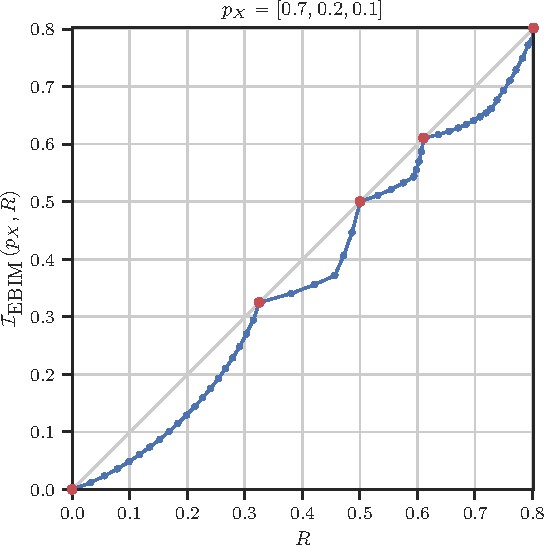
\includegraphics[width=.55\linewidth]{figs/ch3/numerical1.pdf}
    \caption{
        Brute force solutions for $\obj(p_X, R)$ across possible values of $R$ with $p_X = [0.7, 0.2, 0.1]$. Points where $\obj(p_X, R) = R$ are marked with red circles, indicating the 5 possible deterministic mappings (5 possible partitions of $\mathcal{X}$).
    }
    \label{ch3:fig:bruteforce}
\end{figure}
\FloatBarrier

%------------------------------------ Proposed Search Algorithm -------------------------------------
% \newpage
\subsection{Proposed Search Algorithm for Deterministic Mappings}\label{ch3:sec:prposedsearch}
Since iterating over all deterministic mappings is not feasible, one should look for carefully constructed search algorithms to find such mappings with resulting $H(T)$ as close as possible to $R$. 

Without the loss of generality, suppose $p_X = \rvect{p_1, \ p_2, \ \cdots, \ p_n}$ is arranged in a decreasing order. 
Algorithm~\ref{ch3:alg:search} presents a search approach for discovering a deterministic mapping $ T=g(X) $, resulting in $I(X;T)$ that is at most $h(p_2)$ bits away from the optimal $ \obj(p_X, R) $.

% \begin{algorithm}
% \caption{Deterministic EBIM Solver}\label{ch3:alg:search}\vspace{4pt}
% \begin{algorithmic}[1]
%     % \onehalfspacing
%     \Require $p_X, R$
%     \Ensure $\Pxt$
%     \State $\Pxt \gets \text{diag}(p_X)$ \Comment{define $\Pl{0}:= \text{diag}(p_X)$}
%     \For{$i \gets 1$ to $\vert p_X \vert - 1$}
%     \State $\Ps{i} \gets \text{Merge two columns with the smallest sum in } \Pxt$
%     % \State $\Is{i} \gets \ent{\xsum_x \Ps{i}}$
%     \State $\Is{i} \gets \text{Mutual Information imposed by } \Ps{i}$.
%     \State $\Pl{i} \gets \text{Merge two columns with the largest sum in } \Pxt$
%     % \State $\Il{i} \gets \ent{\xsum_x \Pl{i}}$ \label{ch3:alg:Il}
%     \State $\Il{i} \gets  \text{Mutual Information imposed by } \Pl{i}$. \label{ch3:alg:Il}
%     \If{$\Is{i} \leq R$} 
%         \State \Return $\Ps{i}$
%     \ElsIf{$\Il{i} \leq R < \Is{i}$}
%         \State \Return $\Pl{i}$
%     \Else
%         \State $\Pxt \gets \Pl{i}$
%     \EndIf
%     \EndFor
%     \end{algorithmic}
% \end{algorithm}
% \FloatBarrier

\begin{algorithm}[!h]
\caption{Deterministic EBIM Solver}\label{ch3:alg:search}
% \vspace{4pt}
\begin{spacing}{1.2}
\begin{algorithmic}[1]
    % \onehalfspacing
    \Require $p_X, R$
    \Ensure $\Pxt$
    \State $\Pxt \gets \text{diag}(p_X)$ \Comment{define $\Pmerged{0}:= \text{diag}(p_X)$}
    \If{$R \geq H(p_X)$}
        \State \Return $\Pxt$
    \EndIf
    \For{$i \gets 1$ to $\vert p_X \vert - 1$}
        \State $\Pmerged{i} \gets \text{Merge two columns with the largest sum in } \Pxt$.
        \State $\Imerged{i} \gets  I(X;T) \text{ imposed by } \Pmerged{i}$. \label{ch3:alg:Il}
        
        \If{$\Imerged{i} \leq R$}
            \State \Return $\Pmerged{i}$
        \Else
            \State $\Pxt \gets \Pmerged{i}$
        \EndIf
    \EndFor    
\end{algorithmic}
\end{spacing}
\end{algorithm}
\FloatBarrier

% \begin{remark}\label{ch3:rem:searchalg}
Let $n=\vert p_X\vert$. The procedure outlined in Algorithm~\ref{ch3:alg:search} establishes a series of deterministic mappings
$ \Pmerged{0},\, \Pmerged{1},\, \Pmerged{2},\, \cdots,\, \Pmerged{n-1}$,
corresponding to a decreasing sequence of mutual information values 
$ \Imerged{0},\, \Imerged{1},\, \Imerged{2},\, \cdots,\, \Imerged{n-1}$. 
This is done by iteratively merging two elements in $\mathcal{T}$ with the largest probabilities.
% A \textit{hybrid} merger type equates to a largest merger if the compression rate exceeds 2, and to a smallest merger otherwise. The rationale behind this choice will be explained shortly.
The algorithm then picks the mapping with the maximum mutual information that does not exceed $R$. Therefore
\begin{align}
    R - I(X;T) 
    &\leq \max \left\{ \Imerged{0} - \Imerged{1},\; \Imerged{1} - \Imerged{2},\; \cdots,\; \Imerged{n-2} - \Imerged{n-1} \right\} \nonumber \\
    &\leq \maxi \Imerged{i-1} - \Imerged{i} . \label{ch3:eq:detmapbound}
\end{align}    
% \end{remark}

\begin{example}
    For $p_X = \rvect{0.4& 0.2& 0.15& 0.15& 0.1}$, Algorithm~\ref{ch3:alg:search} traverses through the following deterministic mappings, from left to right:
\begin{table}[!h]
\resizebox{\linewidth}{!}{
    $
    \centering
    \arraycolsep=3pt
    \begin{array}{c | c c c c c}
    
        & \Pmerged{0} & \Pmerged{1} & \Pmerged{2} & \Pmerged{3} & \Pmerged{4} \\[5pt] \hline  \rule{0pt}{3\normalbaselineskip}
        \Pxt 
        & \begin{bmatrix}
            .4 & 0   & 0    & 0    & 0  \\
            0   & .2 & 0    & 0    & 0  \\
            0   & 0   & .15 & 0    & 0  \\
            0   & 0   & 0    & .15 & 0  \\
            0   & 0   & 0    & 0    & .1\\
        \end{bmatrix}
        & \begin{bmatrix}
            .4 & 0    & 0    & 0  \\
            .2 & 0    & 0    & 0  \\
            0   & .15 & 0    & 0  \\
            0   & 0    & .15 & 0  \\
            0   & 0    & 0    & .1\\
        \end{bmatrix}
        & \begin{bmatrix} 
            .4  & 0    & 0  \\
            .2  & 0    & 0  \\
            .15 & 0    & 0  \\
            0    & .15 & 0  \\
            0    & 0    & .1\\
        \end{bmatrix}
        & \begin{bmatrix}
            .4   & 0  \\
            .2   & 0  \\
            .15  & 0  \\
            .15  & 0  \\
            0    & .1\\
        \end{bmatrix}
        & \begin{bmatrix}
            .4   \\
            .2   \\
            .15  \\
            .15  \\
            .1  \\
        \end{bmatrix}\\ [28pt]

        I\left(X;T\right) 
        & \ent{p_X} 
        & \ent{\rvect{.6 & .15 & .15& .1}} 
        & \ent{\rvect{.75 & .15 & .1}} 
        & \ent{\rvect{.9 & .1}} 
        & 0\\ \rule{0pt}{0.2\normalbaselineskip}
        
    \end{array}
    $
}
\end{table}
\FloatBarrier

\end{example}


\begin{definition}\label{ch3:def:deltaH}
    Let $\mu'$ be a probability distribution resulted from merging two elements $p > 0$ and $q > 0$ in an original distribution $\mu$, i.e.
    $\mu = \rvect{\cdots & p & \cdots & q & \cdots}$ and $\mu' = \rvect{\cdots & p+q & \cdots}$. Then, the amount of decrease in the entropy from this merge operation is characterized by:
    \begin{align*}
        \DeltaH{p}{q} &= \ent{\mu} - \ent{\mu'} \\
        &= p\log\frac{1}{p} + q\log\frac{1}{q} - (p+q)\log\frac{1}{p+q} \\
        &= p\log\left(1+\frac{q}{p}\right) + q\log\left(1+\frac{p}{q}\right)
    \end{align*}
\end{definition}

\begin{lemma}\label{ch3:lem:DeltaH}
    The following properties hold for the function $\DeltaHsymbol$:
    \begin{enumerate}
        \item $\DeltaH{\cdot}{\cdot}$ is monotonically increasing in both arguments. \label{ch3:lem:DeltaH1}
        \item $\DeltaH{\cdot}{\cdot}$ is concave.
        \item $\DeltaH{p}{1-p} = h(p)$. \label{ch3:lem:DeltaH3}
    \end{enumerate}
\end{lemma}
\begin{proof}
    The properties are derived through straightforward derivative calculations:
    \begin{enumerate}
        \item $\frac{\partial}{\partial p}\DeltaHsymbol = \log (1+q/p) \geq 0$, and 
              $\frac{\partial}{\partial q}\DeltaHsymbol = \log (1+p/q) \geq 0$.
        \item The Hessian of $\DeltaHsymbol$ is negative semidefinite:
        \[
            \mathbf{H}_{\DeltaHsymbol} = \frac{1}{p+q} \begin{bmatrix} 
            -q/p & 1  \\
            1 & -p/q  \\
            \end{bmatrix}
        \]
        with eigenvalues $\lambda_1=0$ and $\lambda_2 = - (\frac{q}{p}+\frac{p}{q})(\frac{1}{p+q}) < 0$.
        \item $\DeltaH{p}{1-p} = -p\log p - (1-p)\log(1-p) = h(p)$.
        
    \end{enumerate}
\end{proof}

\begin{theorem}
    If the output of Algorithm~\ref{ch3:alg:search} yields mutual information $\widehat{I}$, then 
    \[\obj(p_X, R) - \widehat{I} \leq h(p_2),\] where $h(\cdot)$ is the binary entropy function, and $p_2$ denotes the second largest element of $p_X$.
\end{theorem}

\begin{proof}
    For the gap to the optimal objective, $\obj(p_X, R) - \widehat{I}$, we have:
    {\savebox\strutbox{$\vphantom{\dfrac11}$}
    \begin{alignat*}{2}
        \setlength{\arraycolsep}{-10pt}
        &\cmt{\text{Equation (\ref{ch3:eq:objUpper})}} \hspace{2em} \obj(p_X, R) - \widehat{I}                                      
        &&\leq R - \widehat{I} \\
        %
        & \cmt{\text{Equation \eqref{ch3:eq:detmapbound}} }
        &&\leq \maxi \Imerged{i-1} - \Imerged{i} \\
        % 
        &\cmt{\text{Algorithm~\ref{ch3:alg:search}, Line~\ref{ch3:alg:Il}}}
        &&= \maxi \ent{ \xsum_x \Pmerged{i-1} } - \ent{ \xsum_x \Pmerged{i} } \\
        % 
        &\cmt{\text{Definition~\ref{ch3:def:deltaH}}}
        &&= \maxi \DeltaH{\xsum_{k=1}^i p_k}{p_{i+1}} \\
        % 
        &\cmt{\text{Lemma~\ref{ch3:lem:DeltaH}}.\ref{ch3:lem:DeltaH1}}       
        &&\leq \maxi \DeltaH{\xsum_{k=1}^i p_k + \xsum_{k=i+2}^{n} p_k}{p_{i+1}} \\
        % 
        &                                                           
        &&= \maxi \DeltaH{1 - p_{i+1}}{p_{i+1}} \\
        % 
        &\cmt{\text{Lemma~\ref{ch3:lem:DeltaH}}.\ref{ch3:lem:DeltaH3}}       
        &&= \maxi \ h\left(p_{i+1}\right) \\
        % 
        &\cmt{p_2,\, p_3,\, \cdots,\, p_n \leq 0.5}                           
        &&= h(p_2)
    \end{alignat*}
    }
\end{proof}

% Note that the above bound on the optimality of the proposed algorithm is by no means tight, as it does not account for the intermediate distributions $\Ps{i}$.

As discussed in Section~\ref{ch3:sec:relatedworks}, our proposed search method in Algorithm~\ref{ch3:alg:search} is compared with the encoder from Shkel et al. (2017) \cite{shkel2017single}. Our formulation directly imposes an entropy constraint on the code, whereas the encoding scheme by Shkel et al. limits the code by its alphabet size. In their approach, given a code alphabet size, the encoder iterates over all input symbols, assigning each one to a message that has accumulated the smallest total probability up to that point. 

Figure~\ref{ch3:fig:yanina} displays the mutual information obtained for each maximum allowed code rate value, considering two different input distributions. As observed, the two methods yield comparable mutual information in the high-rate regime. However, in the low-rate regime, our proposed algorithm identifies more mappings and thus significantly outperforms the encoder described in \cite{shkel2017single}.

\begin{figure}
    \centering
    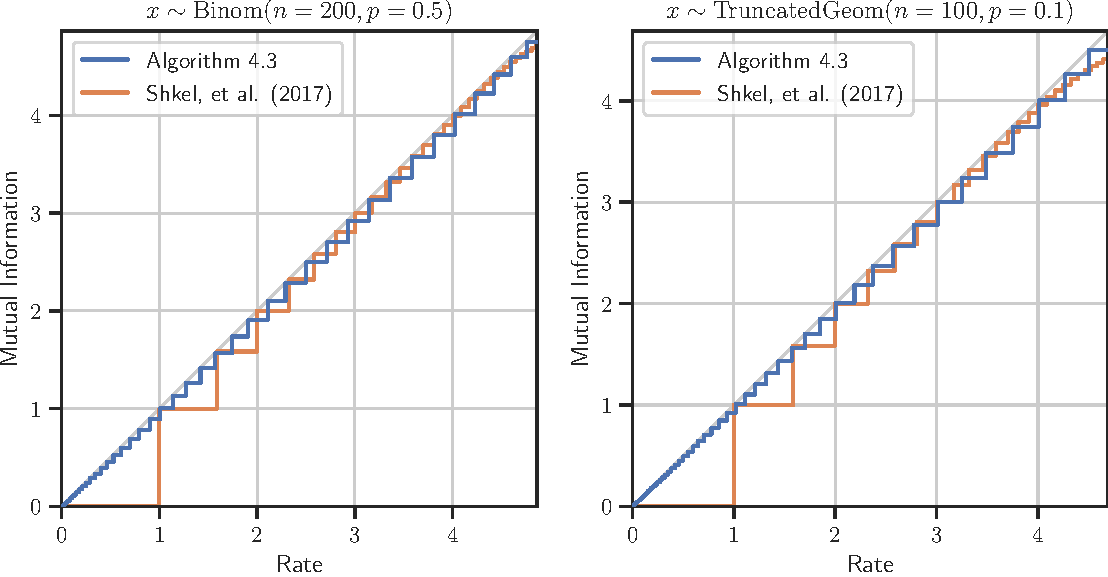
\includegraphics[width=\linewidth]{figs/ch3/yanina.pdf}
    \caption{
        Obtained $I(X;T)$ vs. maximum allowed $H(T)$ for Binomial (left) and Truncated Geometric (right) input distributions.
    }
    \label{ch3:fig:yanina}
\end{figure}
\FloatBarrier

Additionally, note that the couplings generated by Algorithm~\ref{ch3:alg:search} display finer granularity at lower rates. This occurs because the algorithm merges input symbols with the largest probabilities at each iteration. However, as shown in Figure~\ref{ch3:fig:hybrid}, more couplings are generated at higher rates if the merger involves the two elements with the smallest probability. Therefore, a \textit{hybrid} merger strategy optimizes granularity across both low and high rate regimes by performing a largest merger for rates less than \(H(X)/2\) and a smallest merger for rates greater than \(H(X)/2\), as in Figure~\ref{ch3:fig:hybrid} left. 

\begin{figure}[!h]
    \centering
    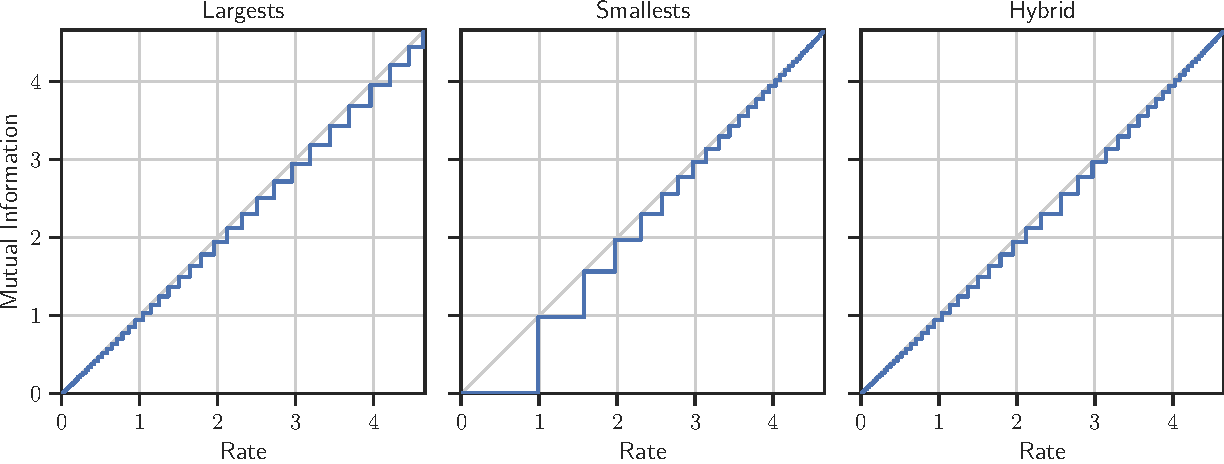
\includegraphics[width=\linewidth]{figs/ch3/hybrid.pdf}
    \caption{
        Iteratively merging two elements in $\mathcal{T}$ with either the largest (left) or smallest (middle) probabilities. A \textit{hybrid} merger (right) equates to a largest merger if the compression rate exceeds 2 and to a smallest merger otherwise.
    }
    \label{ch3:fig:hybrid}
\end{figure}
\FloatBarrier

Algorithm~\ref{ch3:alg:hybrid} demonstrates this hybrid merger strategy.

\begin{algorithm}
\caption{Deterministic EBIM Solver with Hybrid Merger}\label{ch3:alg:hybrid}
% \vspace{4pt}
\begin{algorithmic}[1]
    % \onehalfspacing
    
    \Require $p_X$, $R$
    \Ensure $\Pxt$
    \State $\Pxt \gets \text{diag}(p_X)$
    \If{$R \geq H(p_X)$}
        \State \Return $\Pxt$
    \EndIf
    \For{$i \gets 1$ to $\vert p_X \vert - 1$}
    \If{$R > {H(p_X)} / {2}$}
        \State $\Pmerged{i} \gets \text{Merge two columns with the smallest sum in } \Pxt$.
    \Else
        \State $\Pmerged{i} \gets \text{Merge two columns with the largest sum in } \Pxt$.
    \EndIf
    \State $\Imerged{i} \gets I(X;T) \text{ imposed by } \Pmerged{i}$.
    \If{$\Imerged{i} \leq R$} 
        \State \Return $\Pmerged{i}$
    \Else
        \State $\Pxt \gets \Pmerged{i}$
    \EndIf
    \EndFor
\end{algorithmic}
\end{algorithm}
\FloatBarrier

%------------------------------------ Neighborhood of Deterministic Mappings  -------------------------------------
% \newpage
\subsection{Optimal Coupling Around Deterministic Mappings}\label{ch3:sec:neighborhood}

Section~\ref{ch3:sec:prposedsearch} introduced a greedy algorithm for identifying deterministic mappings with a guaranteed gap from the optimal. In this section, we identify optimal mappings close to any deterministic mapping. This approach will enable us to bridge the gap between the deterministic mappings.

\begin{theorem} \label{ch3:thm:neighbor}
Let $\Pxt$ denoted by a $|\mathcal{X}| \times |\mathcal{T}|$ matrix, defines a deterministic mapping $T = g(X)$, with $ I(X;T)=H(T)=R_g $. We have $ \obj(p_X, R_g) = R_g $, and for small enough $ \epsilon > 0 $:
\begin{enumerate}
    % \item $\obj(p_X, R_g + \epsilon)$ is attained by moving infinitesimal probability mass from the cell with the lowest normalized value, to a new column of $\Pxt$. Normalization is done by dividing each column by its sum.
    \item $\obj(p_X, R_g + \epsilon)$ is achieved as follows:\\
    Normalize the columns by dividing each column by its sum. Then, select the cell with the smallest normalized value and move an infinitesimal probability mass from this cell to a new column of $p_{XT}$ in the same row.
    
    % \item $\obj(p_X, R_g - \epsilon)$ is achieved by transferring an infinitesimal probability mass from the smallest cell in the column with the lowest sum, to the column with the highest sum in $\Pxt$.
    \item $\mathcal{I}_{EBIM}(p_X, R_g - \epsilon)$ is achieved as follows:\\
    Identify the columns with the smallest and largest sums in $p_{XT}$. Select the cell with the smallest value in the column with the lowest sum. Transfer an infinitesimal probability mass from this cell to the column with the highest sum in the same row.

\end{enumerate}
\end{theorem}

\begin{example}    
The following depicts an application of Theorem~\ref{ch3:thm:neighbor}:
\begin{figure}[h] 
    \centering
    \vspace{-5pt}
    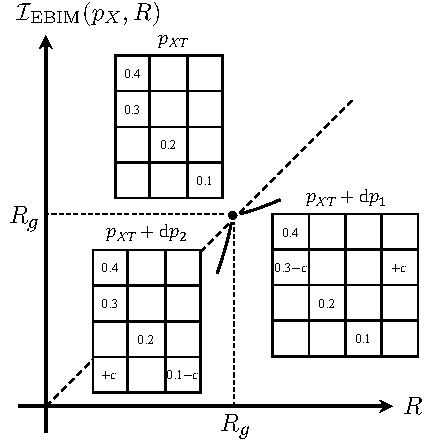
\includegraphics[width=0.3\linewidth]{figs/ch3/didh2.pdf}
    \caption{Optimal solutions in the neighbourhood of a deterministic mapping.}\label{ch3:fig:didh} 
\end{figure}

\FloatBarrier
\end{example}


\begin{proof}
Let us view the joint distribution as a $n\times m$ matrix $\Pxt$. Note that:
\begin{align}
    \label{ch3:eq:g2Pxt}
    \Pxt (x, t) = 
    \begin{cases}
        p_X(x) & t = g(x) \\
        0 & \text{otherwise}
    \end{cases}
\end{align}

For example
\begin{align}
    \label{ch3:eq:example}
    \Pxt = 
    \begin{bmatrix}
        0.4 & 0 & 0 & 0 \\
        0.3 & 0 & 0 & 0 \\
        0 & 0.2 & 0 & 0 \\
        0 & 0 & 0.1 & 0 \\
    \end{bmatrix}
    , \quad g(x) = 
    \begin{cases}
        1, & x = 1, 2 \\
        2, & x = 3 \\
        3, & x = 4 \\
    \end{cases}
\end{align}

Consider a perturbation $\dP \in \mathbb{R}^{n \times m}$ to $ \Pxt $. For $\Pxt + \dP$ to be a valid distribution in $\mathcal{M}$, we need:
\begin{enumerate}
    \item $ \xsum_{t} \dP(x, t) = 0, \ \ \forall x \in \mathcal{X} $ \vspace{-5pt}
    \item $ \dP(x,t) \geq 0, \ \ \forall x, t \ \ \text{s.t.}  \ \ t \neq g(x) $
    \item $ \dP(x,t) \leq 0,  \ \ \forall x, t \ \ \text{s.t.}  \ \ t = g(x) $
\end{enumerate}

We define the set of all such perturbations as $\Omega\subset \mathbb{R}^{n \times m} $. Next, let us define basis perturbations $ \Delta_{x,t} $ for $t \neq g(x)$ as:
\begin{align}
    \left[ \Delta_{x,t} \right]_{ij} = \label{ch3:eq:delta}
    \begin{cases}
      -\dpp, & \text{if} \ \ i=x, \ j=g(x) \\
      +\dpp, & \text{if} \ \ i=x, \ j=t \\
      0, & \text{otherwise}
    \end{cases}
\end{align}

Note that $ \Delta_{x,t} $ represents moving a probability mass of $\dpp$ from non-zero cell $ \left( x, g(x) \right)  $ to empty cell $ \left( x, t \right) $.
For the example in equation \eqref{ch3:eq:example}:
\begin{align*}
    \Delta_{2,3} = 
    \begin{bmatrix}
        0 & 0 & 0 & 0\\
        -\dpp & 0 & +\dpp & 0\\
        0 & 0 & 0 & 0\\
        0 & 0 & 0 & 0\\
    \end{bmatrix}
\end{align*}

The significance of these bases is that any perturbation in $\Omega$ can be represented as:
\begin{align}
    \dP = \sum_{\substack{ x, t \\ t \neq g(x) }} \alpha_{x,t} \ \Delta_{x, t},
\end{align}

with coefficients $ \alpha_{x,t} \geq 0 $. For example:
\[
    \begin{bmatrix}
        0 & 0 & 0 & 0 \\
        -3\dpp & +2\dpp & +\dpp & 0 \\
        0 & 0 & 0 & 0 \\
        0 & 0 & 0 & 0 \\
    \end{bmatrix}
    = 2 \times \Delta_{1, 1} + \Delta_{1, 2}
\]

Realizing  $I_{XT}$, $H_{XT}$, and $H_T$ as functions of a joint distribution, we are interested in calculating the ratio $ \dif{I_{XT}} / \dif{H_T}$ with respect to a perturbation $\dP\in\Omega$ as $\dpp \to 0$ at $\Pxt$. Note that since for any $\dP\in\Omega$, $\dif{H_X}=0$, we have:
\begin{align*}
    \frac{\dif{I_{X,T}}}{\dif{H_T}} 
    = \frac{\dif{H_X} + \dif{H_T} - \dif{H_{X,T}}}{\dif{H_T}} 
    = 1 - \frac{\dif{H_{X,T}}}{\dif{H_T}}. 
\end{align*}
Therefore
\spaced{
\begin{align*}
    \cfrac{\dif{I_{X,T}}}{\dif{H_T}}
    &=  1 - \cfrac{ \dif{H_{X,T}}\left(\Pxt, \dP \right) }{\dif{H_T}\left(\Pxt, \dP \right)} \\
    &=  1 - \cfrac{\dif{H_{X,T}}\left(\Pxt, \ddsum \alpha_{x,t} \ \Delta_{x,t} \right) }{ \dif{H_T}\left(\Pxt, \ddsum \alpha_{x,t} \ \Delta_{x,t} \right)} \\
    &=  1 - \frac{ \ddsum \alpha_{x,t}\ 
    {\dif{H_{X,T}}\left(\Pxt, \Delta_{x,t} \right)}
    }{\ddsum \alpha_{x,t}\ 
    {\dif{H_T}\left(\Pxt, \Delta_{x,t} \right)}
    }
    \numberthis \label{ch3:eq:dIdH}
\end{align*}
}

$\dif{H_{X,T}}\left(\Pxt, \Delta_{x,t} \right)$ represents the amount of change in the joint entropy, when an infinitesimal mass of $\dpp$ is moved from $(x, g(x))$ to $(x, t)$. More precisely, from (\ref{ch3:eq:g2Pxt}) and (\ref{ch3:eq:delta}):
\spaced{
\begin{align*}
    {\dif{H_{X,T}}\left(\Pxt, \Delta_{x,t} \right)} 
    &= H_{X,T} \left( \Pxt + \Delta_{x,t} \right) - H_{X,T} \left( \Pxt \right) \\
    &= \left[ - (p_X(x) - \dpp) \log(p_X(x) - \dpp)  - \dpp \log \dpp \right] - \left[ - p_X(x) \log p_X(x) \right] \\
    &= p_X(x) \log\cfrac{p_X(x)}{p_X(x)-\dpp}  + \dpp \log\cfrac{p_X(x)-\dpp}{\dpp} \\
    &= \dpp + \mathcal{O}(\dpp^2) + \dpp \log\cfrac{p_X(x)}{\dpp} \numberthis \label{ch3:eq:dI}
\end{align*}} 
The last line uses the fact that for small enough $x$, $f(x)=a\log\frac{a}{a-x}=x+\mathcal{O}(x^2).$
Similarly:
\spaced{
\begin{align*}
    \dif{H_{T}}\left(\Pxt, \Delta_{x,t} \right)
    &= H_{T} \left( \Pxt + \Delta_{x,t} \right) - H_{T} \left( \Pxt \right) \\
    \begin{split}
    = \Big[\!-\!\Big( p_T \big( g(x) \big) - \dpp \Big) \log \Big( p_T\big(g(x)\big) - \dpp \Big)\!-\!\Big( p_T(t) + \dpp \Big) \log \Big( p_T(t) + \dpp \Big) \Big] \\
    \hspace{3ex} -\Big[ - p_T \big( g(x) \big) \log  p_T\big(g(x)\big) - p_T(t) \log p_T(t)   \Big] 
    \end{split}
    \\
    &=  p_T\big(g(x)\big) \log\cfrac{p_T\big(g(x)\big)}{p_T\big(g(x)\big)-\dpp}
    + p_T(t) \log\cfrac{p_T(t)}{p_T(t)+\dpp}
    + \dpp \log\cfrac{p_T\big(g(x)\big) - \dpp}{p_T(t) + \dpp} \\
    &= \dpp + \mathcal{O}(\dpp^2) -\dpp + \mathcal{O}(\dpp^2) + \dpp \log\cfrac{p_T\big(g(x)\big)}{p_T(t) + \dpp} \\
    &= \log\cfrac{p_T\big(g(x)\big)}{p_T(t) + \dpp} + \mathcal{O}(\dpp^2) \numberthis \label{ch3:eq:dH}
\end{align*}}

Plugging (\ref{ch3:eq:dI}) and (\ref{ch3:eq:dH}) back to (\ref{ch3:eq:dIdH}), we will get:
\spaced{
\begin{align*}
    \cfrac{\dif{I_{X,T}}}{\dif{H_T}}
    &= 1 - \cfrac{\ddsum \alpha_{x,t} \left[ \dpp + \dpp \log\cfrac{p_X(x)}{\dpp} + \mathcal{O}(\dpp^2) \right]}{\ddsum \alpha_{x,t} \left[ \log \cfrac{p_T\big(g(x)\big)}{p_T(t)+\dpp} + \mathcal{O}(\dpp^2) \right]} \\
    &= 1 - \cfrac{\ddsum \abar_{x,t} \log \cfrac{p_X(x)}{\dpp} }{ \ddsum \abar_{x,t} \log \cfrac{p_T\big( g(x)\big)}{p_T(t)+\dpp}} 
    \numberthis\label{ch3:eq:dIdHlimit}
\end{align*}
}
where $\alpha_{x,t}$ is normalized by: \[ \abar_{x,t} = \frac{\alpha_{x,t}}{\ddsum \alpha_{x,t}}. \]

Let's focus on the limit of (\ref{ch3:eq:dIdHlimit}) when $\dpp\to 0$: If there is any $t\in\mathcal{T}$ with $p_T(t)=0$ and \mbox{$\abar_{x, t}>0$}, the denominator of the second term will grow without bound, otherwise the denominator remains bounded.  Therefore, for the limit of  (\ref{ch3:eq:dIdHlimit})  we have:
\begin{equation}
    \limdp \cfrac{\dif{I_{X,T}}}{\dif{H_T}} 
    =\begin{cases}
        -\infty & \text{if} \hspace{10pt} \abar_{x,t} = 0 \hspace{10pt} \forall t \text{ s.t. }  p_T(t)=0 \\[3pt]
        1-\Big(\doublesum{x}{\ \ p_T(t)=0}\ \abar_{x, t} \Big)^{-1} & \text{if} \hspace{10pt} \exists t: \abar_{x,t}>0 \text{ and } p_T(t)=0 
    \end{cases} \label{ch3:eq:dIdHfinal}
\end{equation}

For $ \dif{H_T}>0 $, we need to find a perturbation (i.e., coefficients $ \alpha_{x,t} $) that maximizes $ \dif{I_{XT}} / \dif{H_T} $. From (\ref{ch3:eq:dIdHfinal}), this means $\exists t\in\mathcal{T}$ with $\abar_{x,t}>0$ and $p_T(t)=0$.
\begin{align*}
    \abar 
    = \argmax_{\abar} \cfrac{\dif{I_{X,T}}}{\dif{H_T}}
    &= \argmax_{\abar} \ 1-\Big(\doublesum{x}{\ \ p_T(t)=0}\ \abar_{x, t} \Big)^{-1} \\[5pt]
    &= \argmax_{\abar} \doublesum{x}{\ \ p_T(t)=0}\ \abar_{x, t} 
\end{align*}

Therefore, $\doublesum{x}{\ \ p_T(t)=0}\ \abar_{x, t}=1$ which means $\abar_{x, t}=0$ if $p_T(t)>0$. In other words, we should only consider perturbations where masses are moved to all-zero columns. Continuing (\ref{ch3:eq:dIdHlimit}):

% \spaced{
\allowdisplaybreaks
\begin{align*}
    \abar 
    &= \argmax_{\abar} \ \frac{\dif{I_{X,T}}}{\dif{H_T}} \\
    &= \argmax_{\abar} \ \ 1 - \cfrac{\doublesum{x}{\ \ p_T(t)=0}  \abar_{x,t} \log \cfrac{p_X(x)}{\dpp} }{ \doublesum{x}{\ \ p_T(t)=0}  \abar_{x,t} \log \cfrac{p_T\big( g(x)\big)}{\dpp}} \\
    &= \argmax_{\abar} \ \ 1 - \cfrac{ - \log\dpp + \doublesum{x}{\ \ p_T(t)=0} \abar_{x,t} \log p_X(x) }{ - \log\dpp + \doublesum{x}{\ \ p_T(t)=0} \abar_{x,t} \log {p_T\big( g(x)\big)}} \\
    &= \argmax_{\abar} \ \ \cfrac{-1}{\log\dpp} 
    \left[ \doublesum{x}{\ \ p_T(t)=0} \abar_{x,t} \log\cfrac{p_T\big( g(x)\big)}{p_X(x)} \right] \\[5pt]
    &= \argmin_{\abar} \ \ \doublesum{x}{\ \ p_T(t)=0} \abar_{x,t} \log\cfrac{p_X(x)}{p_T\big( g(x)\big)}
\end{align*}
% }
This is achieved by selecting
\begin{align}
    \Rightarrow \alpha_{x,t} = 
    \begin{cases}
        1, & x=\argmin\limits_{x'} \cfrac{p_X(x')}{p_T\big(g(x')\big)} \ \text{ and } \ p_T(t)=0  \\
        0, & \text{otherwise}
    \end{cases}
\end{align}
In other words, first, normalize columns in $ \Pxt $ by their sum, then move an infinitesimal probability mass from the cell with the smallest normalized value to an all-zero column. It is easy to confirm that $\dif{H}_T > 0$ for such a perturbation. For the example distribution in (\ref{ch3:eq:example}):
\begin{align}
    \Pxt + \dP = 
    \begin{bmatrix}
        0.4 & 0 & 0 & 0 \\
        0.3-\dpp & 0 & 0 & \dpp \\
        0 & 0.2 & 0 & 0 \\
        0 & 0 & 0.1 & 0 \\
    \end{bmatrix}
\end{align}

On the other hand, for $ \dif{H_T}<0 $, we need to find a perturbation (i.e., coefficients $ \alpha_{x,t} $) that minimizes $ \dif{I_{XT}} / \dif{H_T} $. From (\ref{ch3:eq:dIdHfinal}), this means $\abar_{x,t} = 0$ for all $t\in\mathcal{T}$ that $p_T(t)=0$. Therefore, as in (\ref{ch3:eq:dIdHlimit}):

\spaced{
\begin{align*}
    \abar 
    &= \argmin_{\abar} \ \ \frac{\dif{I_{X,T}}}{\dif{H_T}} \\[5pt]
    &= \argmin_{\abar} \ \ 1 - \cfrac{\ddsum \abar_{x,t} \log \cfrac{p_X(x)}{\dpp} }{ \ddsum \abar_{x,t} \log \cfrac{p_T\big( g(x)\big)}{p_T(t)}} \\[5pt]
    &= \argmin_{\abar} \ \ 1 - \cfrac{-\log\dpp + \ddsum \abar_{x,t} \log {p_X(x)} }{ \ddsum \abar_{x,t} \log \cfrac{p_T\big( g(x)\big)}{p_T(t)}} \\
    &= \argmin_{\abar} \  { \ddsum \abar_{x,t} \log \cfrac{p_T\big( g(x)\big)}{p_T(t)}}
\end{align*}}
This is achieved by selecting
\begin{align}
    \Rightarrow \abar_{x,t} = 
    \begin{cases}
        1, & x=\argmin\limits_{x'} {p_T\big(g(x')\big)} \ \text{ and } \ t = \argmax\limits_{t'} p_T(t')  \\
        0, & \text{otherwise}
    \end{cases}
\end{align}
In other words, moving an infinitesimal probability mass from the smallest column to the largest column of $ \Pxt $. It is easy to confirm that $\dif{H}_T < 0$ for such a perturbation. For the example distribution of (\ref{ch3:eq:example}):
\begin{align}
    \Pxt + \dP = 
    \begin{bmatrix}
        0.4 & 0 & 0 & 0 \\
        0.3 & 0 & 0 & 0 \\
        0 & 0.2 & 0 & 0 \\
        \dpp & 0 & 0.1 -\dpp & 0 \\
    \end{bmatrix}
\end{align}

\end{proof}

While Algorithm~\ref{ch3:alg:search} effectively identifies deterministic mappings that produce mutual information close to the budget $R$, Theorem~\ref{ch3:thm:neighbor} can help bridge the remaining gap. More specifically, one can begin with a deterministic mapping and use two probability mass transformations outlined in Theorem~\ref{ch3:thm:neighbor} to navigate across the $I-R$ plane. 

\begin{figure}[h!]
    \centering
    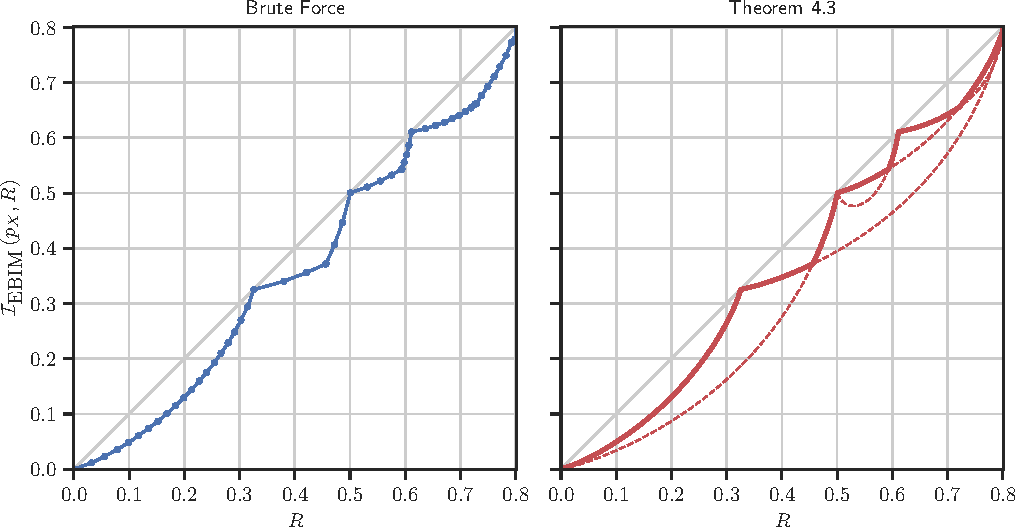
\includegraphics[width=1\linewidth]{figs/ch3/numerical_theorem1.pdf}
    \caption{
    Solutions to the EBIM problem for $p_X=[0.7, 0.2, 0.1]$. Left: brute force solution. Right: Application of the transformations from Theorem~\ref{ch3:thm:neighbor} to each deterministic mapping (dashed lines) and selection of solutions with maximal mutual information for each $R$ value (thick solid line). This strategy effectively recovers optimal solutions, aligning with those found by brute force in this case.
    }
    \label{ch3:fig:numericalvstheorem}
\end{figure}
% \FloatBarrier

Figure~\ref{ch3:fig:numericalvstheorem} illustrates this strategy; for $p_X=[0.7,\ 0.2,\ 0.1]$, identifying all 5 possible deterministic mappings is straightforward. Applying the transformations from Theorem~\ref{ch3:thm:neighbor} then yields various solutions across the $I-R$ plane (represented by dashed lines). Subsequently, one can select the solution that maximizes mutual information for any given value of $R$ (highlighted with a thick solid line), thus producing a comprehensive solution for every value of $R$. As demonstrated in Figure~\ref{ch3:fig:numericalvstheorem}, this strategy recovers the optimal solutions, as determined by brute force, for the simple case of an input alphabet of three. However, the optimality of this approach, while effective, remains a conjecture.

%------------------------------------ Application: Markov Coding Game with Rate Limit  -------------------------------------
% \clearpage
\section{Application: Markov Coding Game with Rate Limit} \label{ch3:sec:mcg}

Markov Coding Games (MCGs) \cite{sokota2022communicating} represent a type of multi-player decentralized Markov Decision Process (MDP) that include the following components: a source, an agent, a Markov decision process, and a receiver. A Markov Coding Game unfolds over four distinct steps:  In the first step, the agent receives a private message from the source, where it is responsible for indirectly conveying the message to the receiver. In the second step, the sender engages in a Markov decision process episode. Next, the receiver observes the sender’s MDP trajectory. The final step involves the receiver attempting to decode the original message from the observed trajectory. The combined reward for both the sender and receiver in this game is determined by a combination of the total rewards accumulated during the MDP episode and a factor that indicates the accuracy of the receiver in decoding the message.

MCGs are particularly interesting due to their ability to extend the scope of several critical frameworks. A prime example is referential games, where a sender aims to communicate a message to a receiver through low-cost or inconsequential actions, known as cheap talk, which don’t affect the game’s transition or reward dynamics. MCGs can be seen as an expansion of referential games, incorporating scenarios where the sender’s actions might have associated costs.

We will consider a natural extension to Markov Coding Games, where the link from the source to the agent is rate-limited. This means, contrary to the original setting in \cite{sokota2022communicating}, the agent does not fully observe the message at each MDP round, but will receive a compressed version of the message iteratively, and in turn, encodes information about the message in the MDP trajectory for the receiver.


\subsection{Backgrounds and Notations}
\paragraph{Markov Decision Process}  MDPs are represented by the tuple notation $(\mathcal{S}, \mathcal{A}, \mathcal{R}, \mathcal{T})$, where $\mathcal{S}$ is the state space, $\mathcal{A}$ denoted the action space, $\mathcal{R}: \mathcal{S} \times \mathcal{A} \rightarrow \mathbb{R}$ defines the reward function, and $\mathcal{T}: \mathcal{S} \times \mathcal{A} \rightarrow \mathcal{P}(\mathcal{S})$ represents the transition function. The way an agent interacts with an MDP is determined by its policy $\pi: \mathcal{S} \rightarrow \mathcal{P}(\mathcal{A})$, which assigns distributions over actions for each state. Our main focus is on episodic MDPs, which terminate after a limited sequence of transitions. The sequence of states and actions, called a trajectory, is recorded as $z = (s_0, a_0, \ldots, s_T)$. The total rewards accrued throughout a sequence is $R(z) = \sum_t \gamma^t R(s_t, a_t)$, where $0<\gamma<1$ is the reward discount factor. The primary aim of an MDP is to devise a policy that maximizes the expected cumulative reward $\mathbb{E}[R(Z) | \pi]$.

\paragraph{Maximum Entropy Reinforcement Learning} a policy that exhibits a high degree of randomness is preferred in certain situations. Under these circumstances, the maximum-entropy RL objective
\begin{align}
    \max_{\pi} \mathbb{E}_{\pi} \left[ \sum_{t} R(S_t, A_t) + \beta H(A_t | S_t) \right] \label{ch3:eq:maxentrl}
\end{align}

serves as a compelling substitute to the conventional goal of maximizing expected aggregate rewards \cite{ziebart2008maximum}. This objective trades off expected returns with conditional entropy of the selected policy, modulated by the temperature hyperparameter $\beta$. A generalization of the Q-value iteration method for maximum-entropy RL objective (also known as soft Bellman equation \cite{sutton2018reinforcement}) is shown in Algorithm~\ref{ch3:alg:softq}.

\begin{algorithm}
\caption{Soft Q-Value Iteration}\label{ch3:alg:softq}
\begin{algorithmic}[1]
\State \textbf{Input:} MDP, $\beta$
\State \textbf{Initialize:} $\pi_0$ to any policy
\State $i \gets 0$
\Repeat
    \State $Q^{i+1}_{\text{soft}}(s,a) \gets R(s,a) + \gamma \sum_{s'} \text{Pr}(s'|s,a) \ \stackMath\stackunder[0.1pt]{\widetilde{\max}_\beta}{_{a'}} \ Q^{i}_{\text{soft}}(s',a')$
    \State $i \gets i + 1$
\Until{$\|Q^{i}_{\text{soft}}(s,a) - Q^{i-1}_{\text{soft}}(s,a)\|_{\infty} \leq \epsilon$}
\State \textbf{Extract policy:} $\pi_{\text{greedy}}(\cdot |s) = \text{softmax}\left(\altfrac{Q^{i}_{\text{soft}}(s,\cdot)}{\beta}\right)$
\end{algorithmic}
\end{algorithm}


The soft maximum operator is defined as $\stackMath\stackunder[0.1pt]{\widetilde{\max}_\beta}{_a} \ Q(s,a) = \beta\log\sum_a \exp \left( \frac{Q(s,a)}{\beta} \right)$.

\paragraph{Markov Coding Games with Rate Limit} 
% Informally, the goal of an agent in a Markov Coding Game is to maximize the rewards from an MDP, and at the same time, encode as much information as possible about a message on the trajectory. 
Following \cite{sokota2022communicating}, we define a rate-limited MCG as a tuple $\langle (\mathcal{S},  \mathcal{A}, \mathcal{T}, \mathcal{R}), \mathcal{M}, \mu, \zeta, R \rangle$, where \((\mathcal{S}, \mathcal{A}, \mathcal{T}, \mathcal{R})\) is a Markov decision process, \(\mathcal{M}\) is a set of messages, \(\mu\) is the prior distribution over messages \(\mathcal{M}\), \(\zeta\) is a non-negative real number we call the message priority, and finally, $R$ is the communication rate limit between the source and the agent. The goal of the agent is to maximize the expected weighted sum of the MDP payoff and the receiver’s accuracy. An MCG proceeds in the following steps:
\begin{enumerate}
    \item  Message \(M \sim \mu\) is sampled from the prior over messages at the source.
    \item Based on the selected message $M$ and the history of the MDP episode, the source generates and transmits signal $T$ to the agent, adhering to the rate limit $R$.
    \item The Agent uses a conditional policy $\pi_{|T}$, which takes current state \(s \in \mathcal{S}\) and received signal \(T \) as input and outputs distributions over MDP actions \(\mathcal{P}(\mathcal{A})\), to generate the next action $a$. 
    \item After repeating steps 2 and 3, the agents’ terminal MDP trajectory \(Z\) is given to the receiver as an observation.
    \item The receiver uses the terminal MDP trajectory $Z$ to output a distribution over messages \(\mathcal{P}(\mathcal{M})\) estimating the message \(\hat{M}\).
\end{enumerate}

The objective of the agents is to maximize the expected weighted sum of the MDP reward and the accuracy of the receiver’s estimate \(\mathbb{E} [\mathcal{R}(Z) + \zeta\mathbb{I}[M = \hat{M}] ]\). Optionally,
If a suitable distance function exists, instead, the objective can also be adjusted to minimize the difference between the actual message and the guess. A diagram of the structure MCG with rate limit is shown in Figure \ref{ch3:fig:mcg}.

\begin{figure}[h] 
    \centering 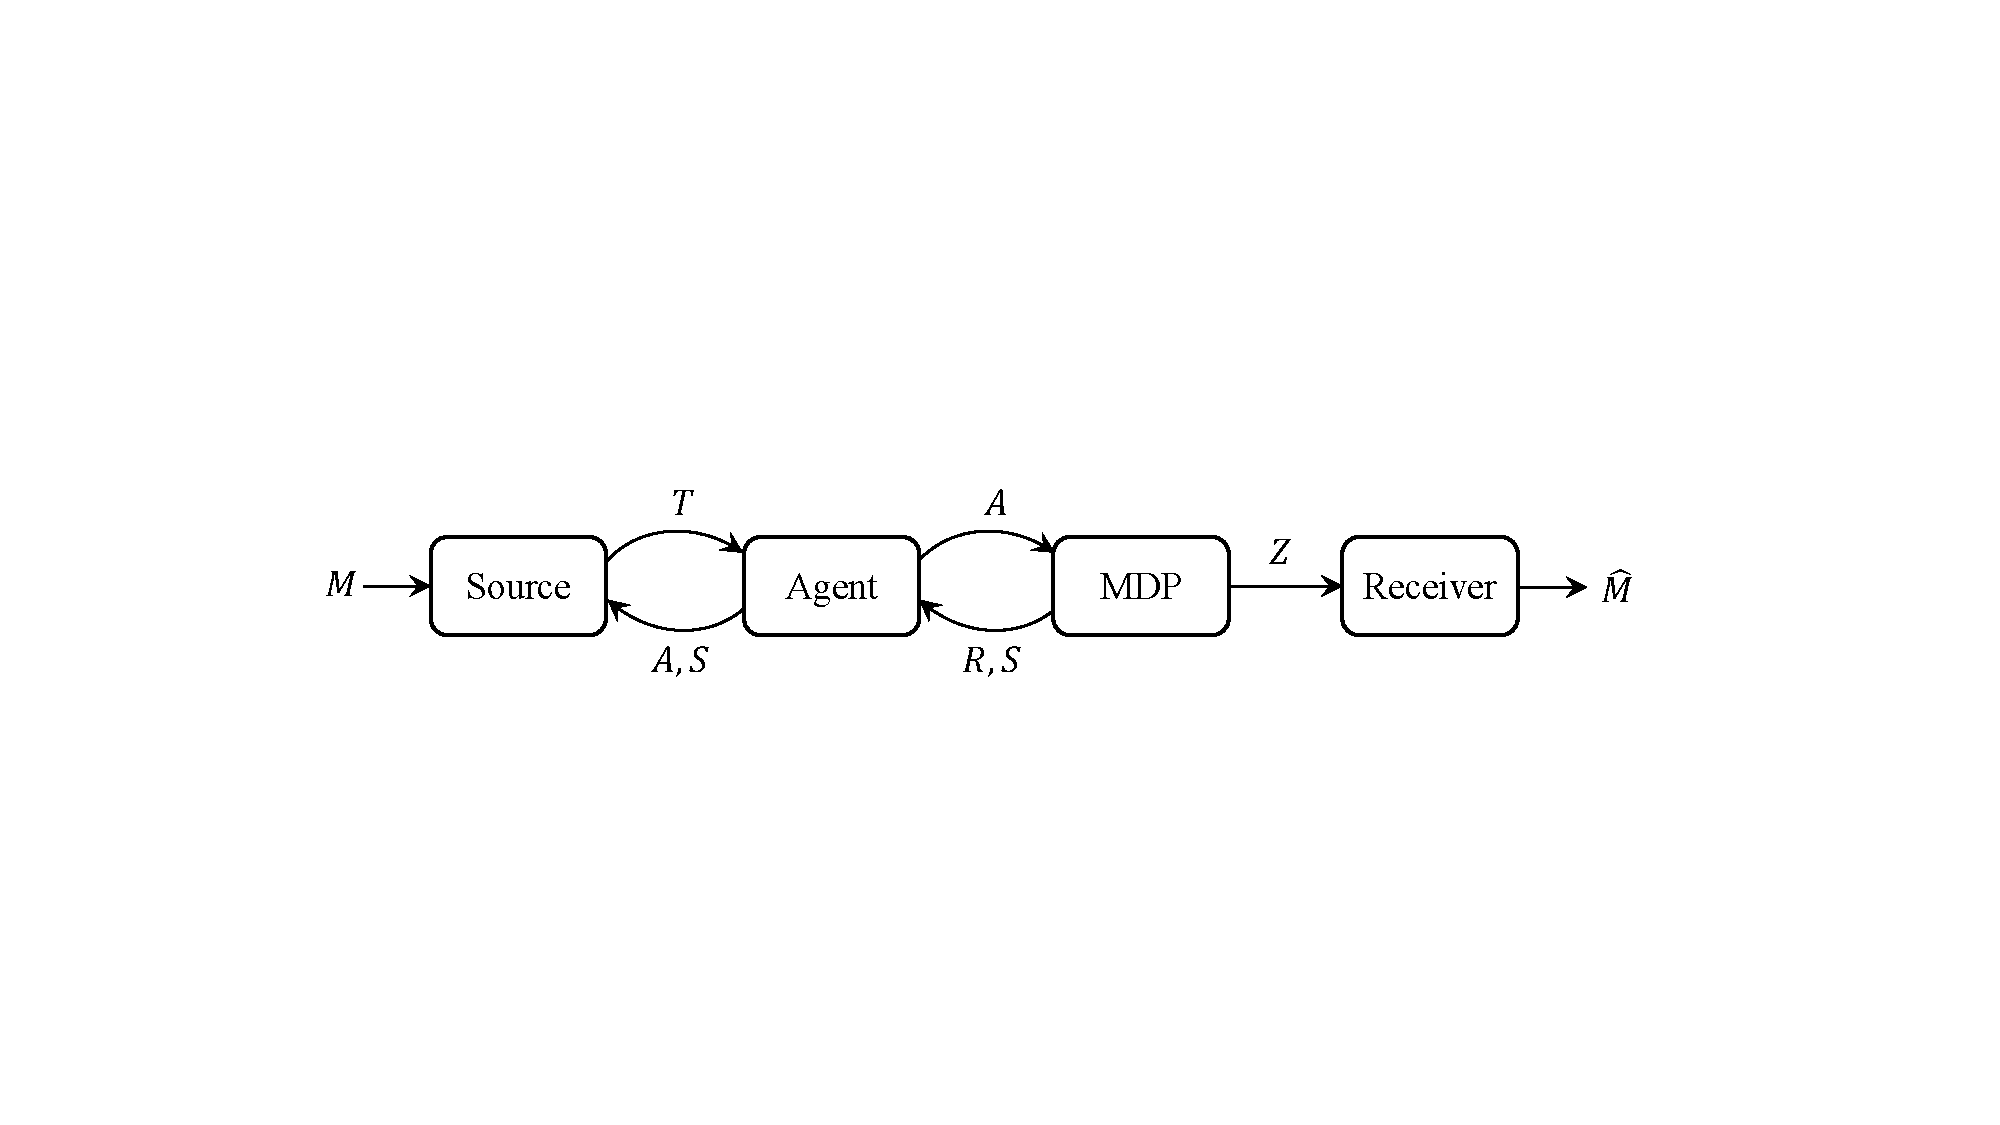
\includegraphics[width=0.9\linewidth]{figs/ch3/MGC.pdf}
    \caption{The structure of a Markov Coding Game with Rate Limit.}\label{ch3:fig:mcg} 
\end{figure}

\subsection{Method Description}\label{ch3:sec:mgcmethod}

\paragraph{Marginal Policy} 
Following \cite{sokota2022communicating}, before execution, we first derive a marginal policy $\pi$ for the MDP, based on the Maximum-Entropy objective outlined in Equation (\ref{ch3:eq:maxentrl}). The value of $\beta$ in the Maximum-Entropy objective needs to be determined in accordance with the message priority $\zeta$ of the MGC. Note that this marginal policy does not depend on the choice of a specific message. By introducing stochasticity into this policy, we can encode information about the message into the selection of actions at each step during runtime

\paragraph{Step 1 - Source: Message Compression}
At the beginning of each round, given the updated message belief $p_M$, the source compresses the message to generate the signal $T$, adhering to the source-agent rate limit $R$, by solving \eqref{ch3:eq:obj}. The source then transmits the signal $T$ to the agent. Subsequently, after observing the action taken by the agent, the source updates the message belief for the next round. Algorithm \ref{ch3:alg:source} outlines the steps taken by the source.

\begin{algorithm}[h]
\caption{Source}\label{ch3:alg:source}
\begin{algorithmic}[1]
    \State \textbf{Input}: marginal policy $\pi$, message prior $\mu$, Rate $R$, initial MDP state $s^0$
    \State Observe message $m \sim \mu$
    \State initialize message belief $p_M \gets \mu$
    \State initialize state $s \gets s^0$
    \While{Source's turn}
        \State $p_{MT}$ $\gets$ \texttt{compress}($p_M$, $R$)
        \State $t \sim p_{T|M}(m)$ \Comment{\textit{{\small In our method, $p_{T|M}$ represent a function.}}}
        \State \textbf{Send} $t$ to the agent.
        
        \Statex \ \ \ \ \textit{//repeating agent's actions to update message belief:}
        \State $p_{T} \gets \sum_{m'} p_{MT}(m', \cdot)$ 
        \State $p_{TA}$ $\gets$ \texttt{min\_ent\_coupling}($p_T$, $\pi(s)$)
        \State $p_{MA} \gets \sum_{t'} p_{MT}(\cdot, t') \ p_{A|T}(t') $
        \State $a, s \gets$ \textbf{Observe} action and next state from MDP.
        \State $p_{M} \gets p_{M|A}(a)$
    \EndWhile
\end{algorithmic}
\end{algorithm}

\paragraph{Step 2 - Agent: Minimum Entropy Coupling}
As illustrated in Algorithm \ref{ch3:alg:agent}, at each round, upon receiving the signal $T$, the agent constructs a conditional policy $\pi_{|T}$ by performing minimum entropy coupling between the action distribution from the marginal policy \(\pi(s)\) with the signal distribution \(p_T\). Subsequently, the next action is sampled from the conditional policy, \(a \sim \pi_{|T}\). Finally, the agent updates the message belief based on the chosen action.

\begin{algorithm}[h]
\caption{Agent}\label{ch3:alg:agent}
\begin{algorithmic}[1]
    \State \textbf{Input}: marginal policy $\pi$, message prior $\mu$, Rate $R$, initial MDP state $s^0$
    \State initialize message belief $p_M \gets \mu$
    \State initialize state $s \gets s^0$
    \While{Agent's turn}
        \State $p_{MT}$ $\gets$ \texttt{compress}($p_M$, $R$)
        \State \textbf{Receive} $t$ from the source.
        \State $p_{T} \gets \sum_{m'} p_{MT}(m', \cdot)$
        \State $p_{TA}$ $\gets$ \texttt{min\_ent\_coupling}($p_T$, $\pi(s)$)
        \State $\pi_{|T} \gets p_{A|T}(t)$
        \State $a \sim \pi_{|T}$
        \State $s \gets $ commit action $a$ to MDP.
        \State $p_{MA} \gets \sum_{t'} p_{MT}(\cdot, t') \ p_{A|T}(t') $
        \State $p_{M} \gets p_{M|A}(a)$
    \EndWhile
    \end{algorithmic}
\end{algorithm}

\paragraph{Receiver: Decoding the Message}
Given the agent’s MDP trajectory, the receiver mirrors the actions of the source and agent to update the message belief at each step. As outlined in Algorithm \ref{ch3:alg:receiver}, the process begins with the receiver compressing the message based on the current message belief. This is followed by performing minimum entropy coupling between the marginal policy and the distribution of the compressed message.

\begin{algorithm}[h!]
\caption{Receiver} \label{ch3:alg:receiver}
\begin{algorithmic}[1]
    \State \textbf{Input}: MDP trajectory $z$, marginal policy $\pi$, message prior $\mu$, Rate $R$, initial MDP state~$s^0$
    \State initialize message belief $p_M \gets \mu$
    \State initialize state $s \gets s^0$
    \For{$s, a \in z$}
        \State $p_{MT}$ $\gets$ \texttt{compress}($p_M$, $R$)
        % \State \textbf{Receive} $t$ from the source.
        
        \State $p_{T} \gets \sum_{m'} p_{MT}(m', \cdot)$
        \State $p_{TA}$ $\gets$ \texttt{min\_ent\_coupling}($p_T$, $\pi(s)$)
    
        % \State $\pi_{|T} \gets p_{A|T}(t)$
        % \State $a \sim \pi_{|T}$
        % \State $s \gets $ commit action $a$ to MDP.
    
        \State $p_{MA} \gets \sum_{t'} p_{MT}(\cdot, t') \ p_{A|T}(t') $
        \State $p_{M} \gets p_{M|A}(a)$
    \EndFor
    \State estimated message $\hat{m} \gets \arg\max_{m'} p_M(m')$
\end{algorithmic}
\end{algorithm}


% \clearpage
\section{Experiments}\label{ch3:sec:exp}

\subsection{Minimum Entropy Coupling with Bottleneck}

As discussed in Section~\ref{ch3:sec:introduction}, optimizing the encoder and decoder separately for the Minimum Entropy Coupling with Bottleneck (MEC-B) problem, as outlined in \eqref{ch3:eq:mecb}, involves first designing the encoder by solving the Entropy-Bounded Information Maximization (EBIM) in \eqref{ch3:eq:obj}. This is followed by optimizing the decoder using Minimum Entropy Coupling (MEC) between the code distribution (derived from the previous step) with the output distribution.

To illustrate the couplings generated, we apply the MEC-B framework to inputs and outputs that are uniformly distributed across an alphabet of size 30. For EBIM, we only search for deterministic mappings using Algorithm~\ref{ch3:alg:search}, while for MEC, we employ the max-seeking method outlined in Algorithm~\ref{ch3:alg:maxseekMEC}.

Figure~\ref{ch3:fig:couplingvscomp} illustrates the generated couplings for varying encoder compression rates, defined by the ratio of the entropy of the input $H(X)$ to the allowed code budget $H(T)$. Greater compression rates are observed to lead to larger entropy couplings; moving from completely deterministic mappings to increasingly stochastic ones.

\begin{figure}[b!]
    \centering
    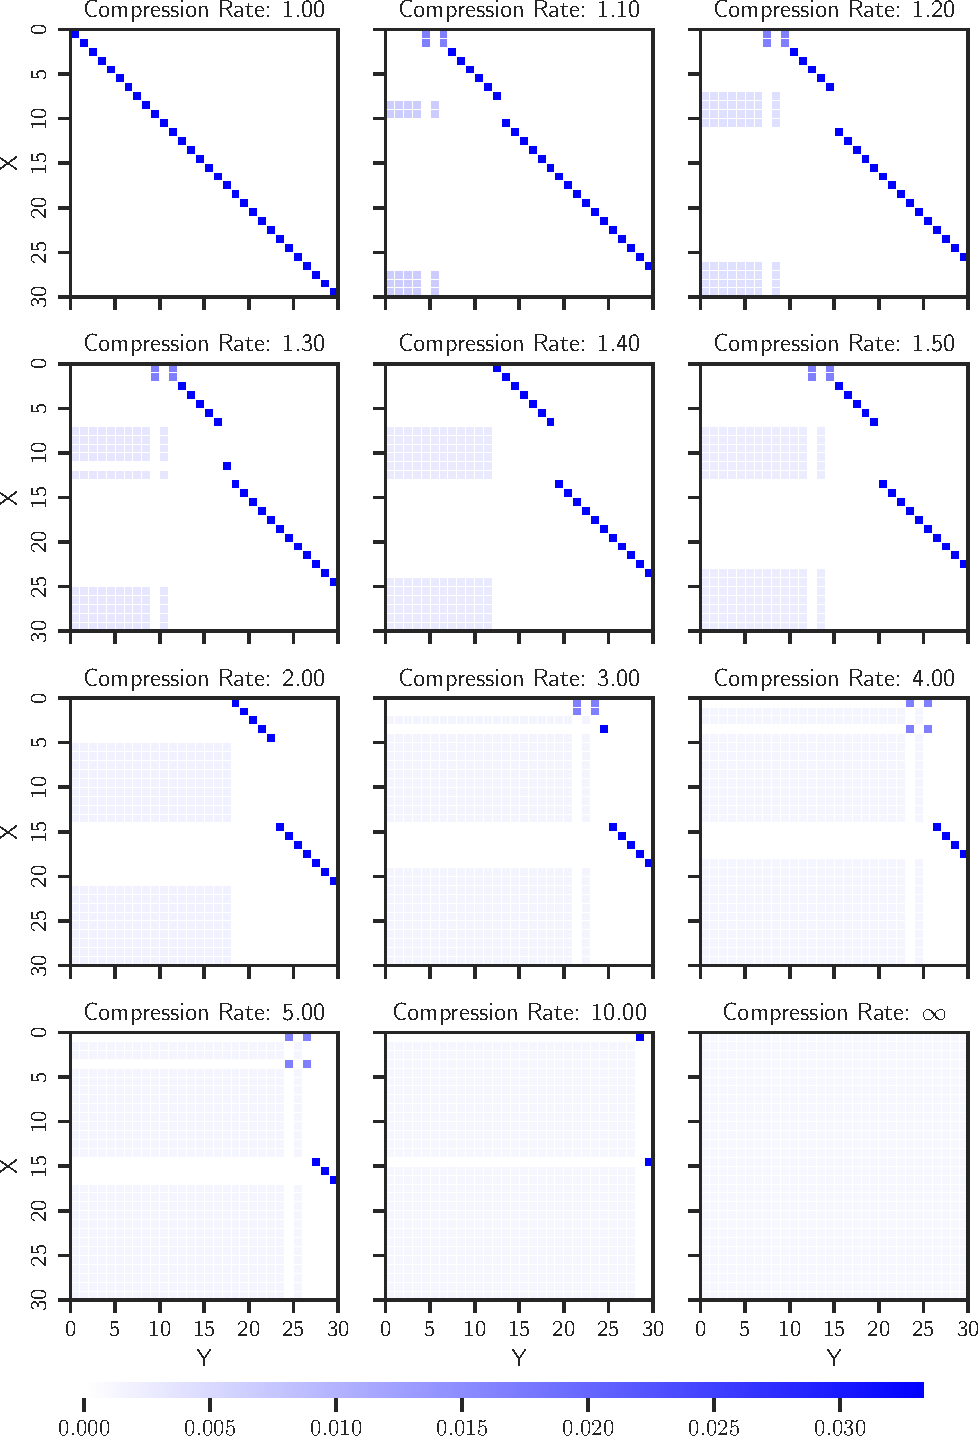
\includegraphics[width=.9\linewidth]{figs/ch3/couplingvscomp.pdf}
    \caption{
        Generated couplings in MEC-B formulation \eqref{ch3:eq:mecb}, for uniform input and output distributions. The compression rate is defined as $H(X)/R$. Higher compression rates lead to more stochastic couplings with increased entropy.
    }
    \label{ch3:fig:couplingvscomp}
\end{figure}
\FloatBarrier

\subsection{Markov Coding Games with Rate Limits}

This section presents the experimental results of the method described in Section~\ref{ch3:sec:mgcmethod}, applied to Markov Coding Games. For our experiments, we utilize a simple environment known as \textit{Grid World}, for the Markov Decision Process. In this setup, the agent is placed on an \(8 \times 8\) grid and, at each step, can move left, right, up, and down. The primary objective for the agent is to navigate from the starting cell to the goal cell to receive a reward of \(1\), while avoiding a trap cell with a reward of \(-1\).
Also, the environment is noisy; even if the agent decides to move in a specific direction, the environment might, with a certain noise probability, force a move in a direction \(90^\circ\) off the intended path. The rewards received are discounted by a factor of \(0.95\). Finally, the receiver has to decode a message, uniformly chosen from an alphabet of size 1024, given the final trajectory of the agent. Figure~\ref{ch3:fig:gwbeta0} illustrates the Grid World used in this experiment and depicts a trajectory taken by the agent.

\begin{figure}[h!]
    \centering
    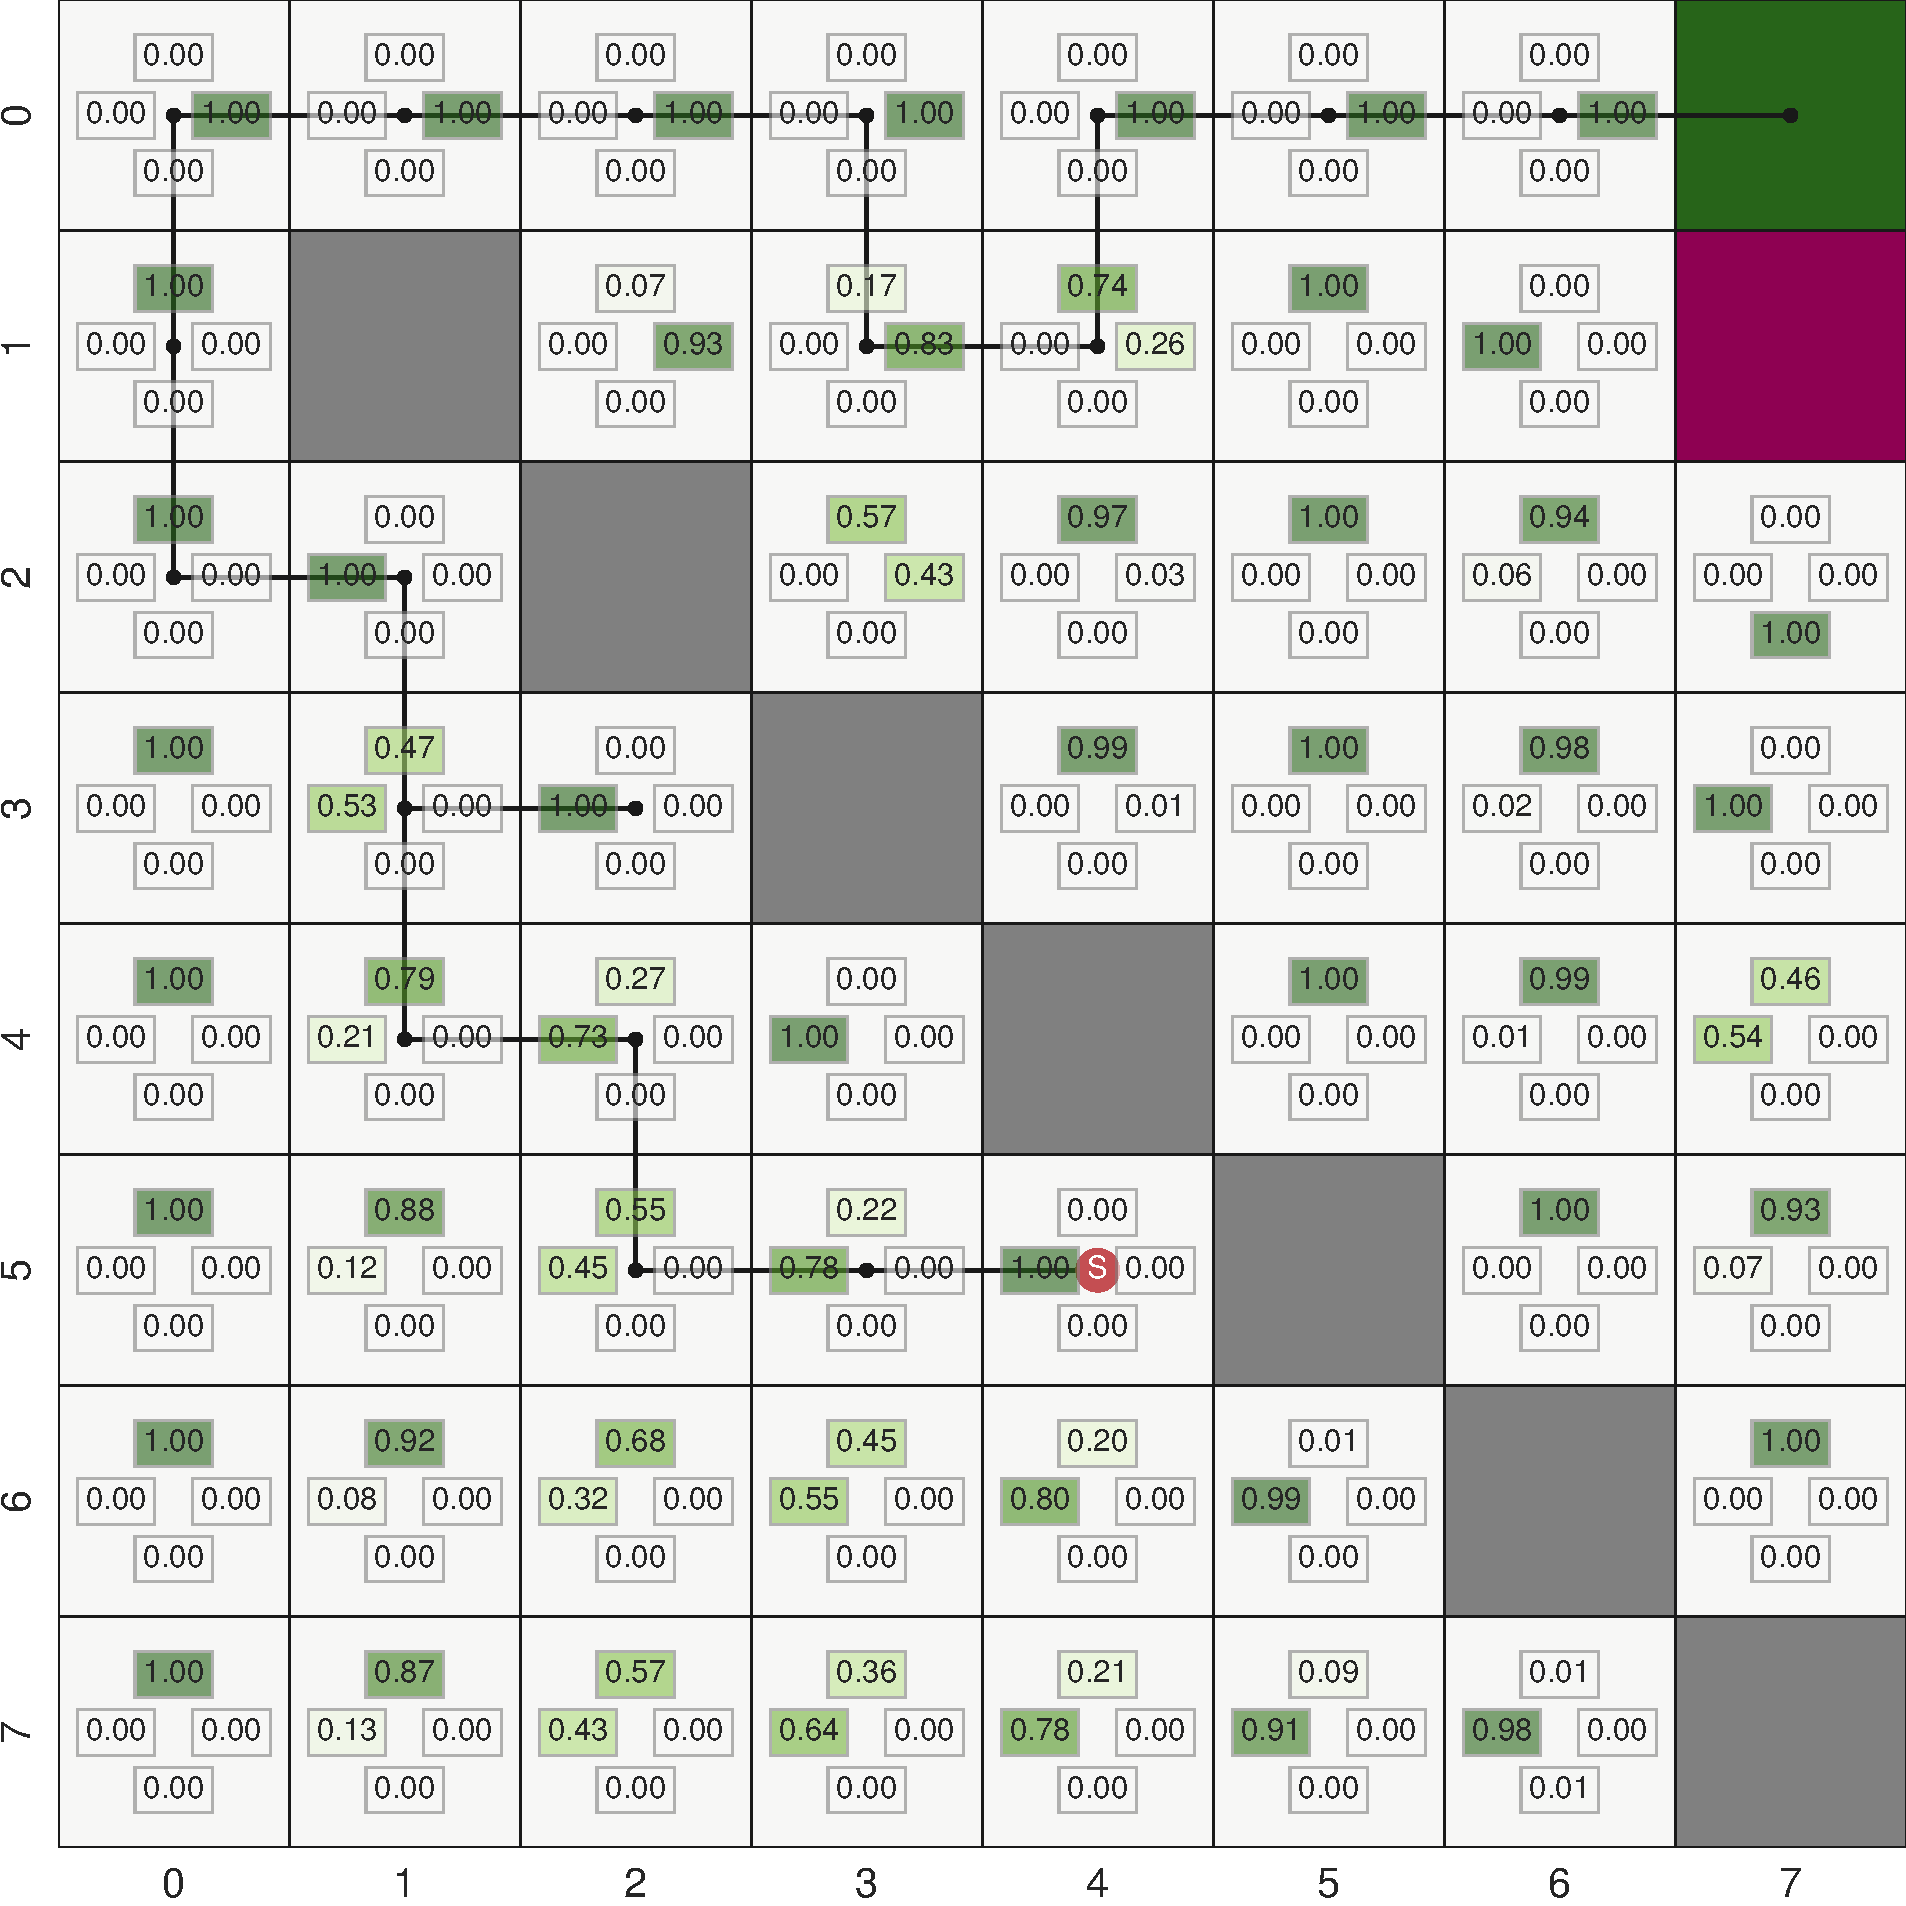
\includegraphics[width=0.75\linewidth]{figs/ch3/gw_beta0.pdf}
    \caption{The Grid World Setup used in the experiments. The starting cell is depicted by a red circle, while the goal, trap, and obstacle cells are colored green, red, and grey, respectively. Additionally, a non-deterministic policy is demonstrated through the probabilities of actions in each direction within each cell. The path taken by the agent is traced in black. Note that due to the noisy environment, the agent may move in directions not explicitly suggested by the policy.
    }\label{ch3:fig:gwbeta0}
\end{figure}
% \FloatBarrier

The marginal policy is learned through Soft Q-Value iteration, as described in Algorithm~\ref{ch3:alg:softq}. By increasing the value of \(\beta\) in Equation~\eqref{ch3:eq:maxentrl}, we induce more randomness into the marginal policy. Consequently, higher values of \(\beta\) lead to an increase in the total number of steps taken by the agent to reach the goal, resulting in a more heavily discounted reward. Conversely, as the entropy of actions at each state is increased, there is an increase in the mutual information between the actions and the compressed message during the minimum entropy coupling at each step. This dynamic establishes a fundamental trade-off between the MDP reward and the accuracy of the message decoded by the receiver, through the adjustment of \(\beta\). Figure~\ref{ch3:fig:twobetas} shows two policies learned by high and low values of $\beta$.

\begin{figure}[ht]
    % \vspace{-1em}
    \centering
    \begin{minipage}[b]{0.48\linewidth}
        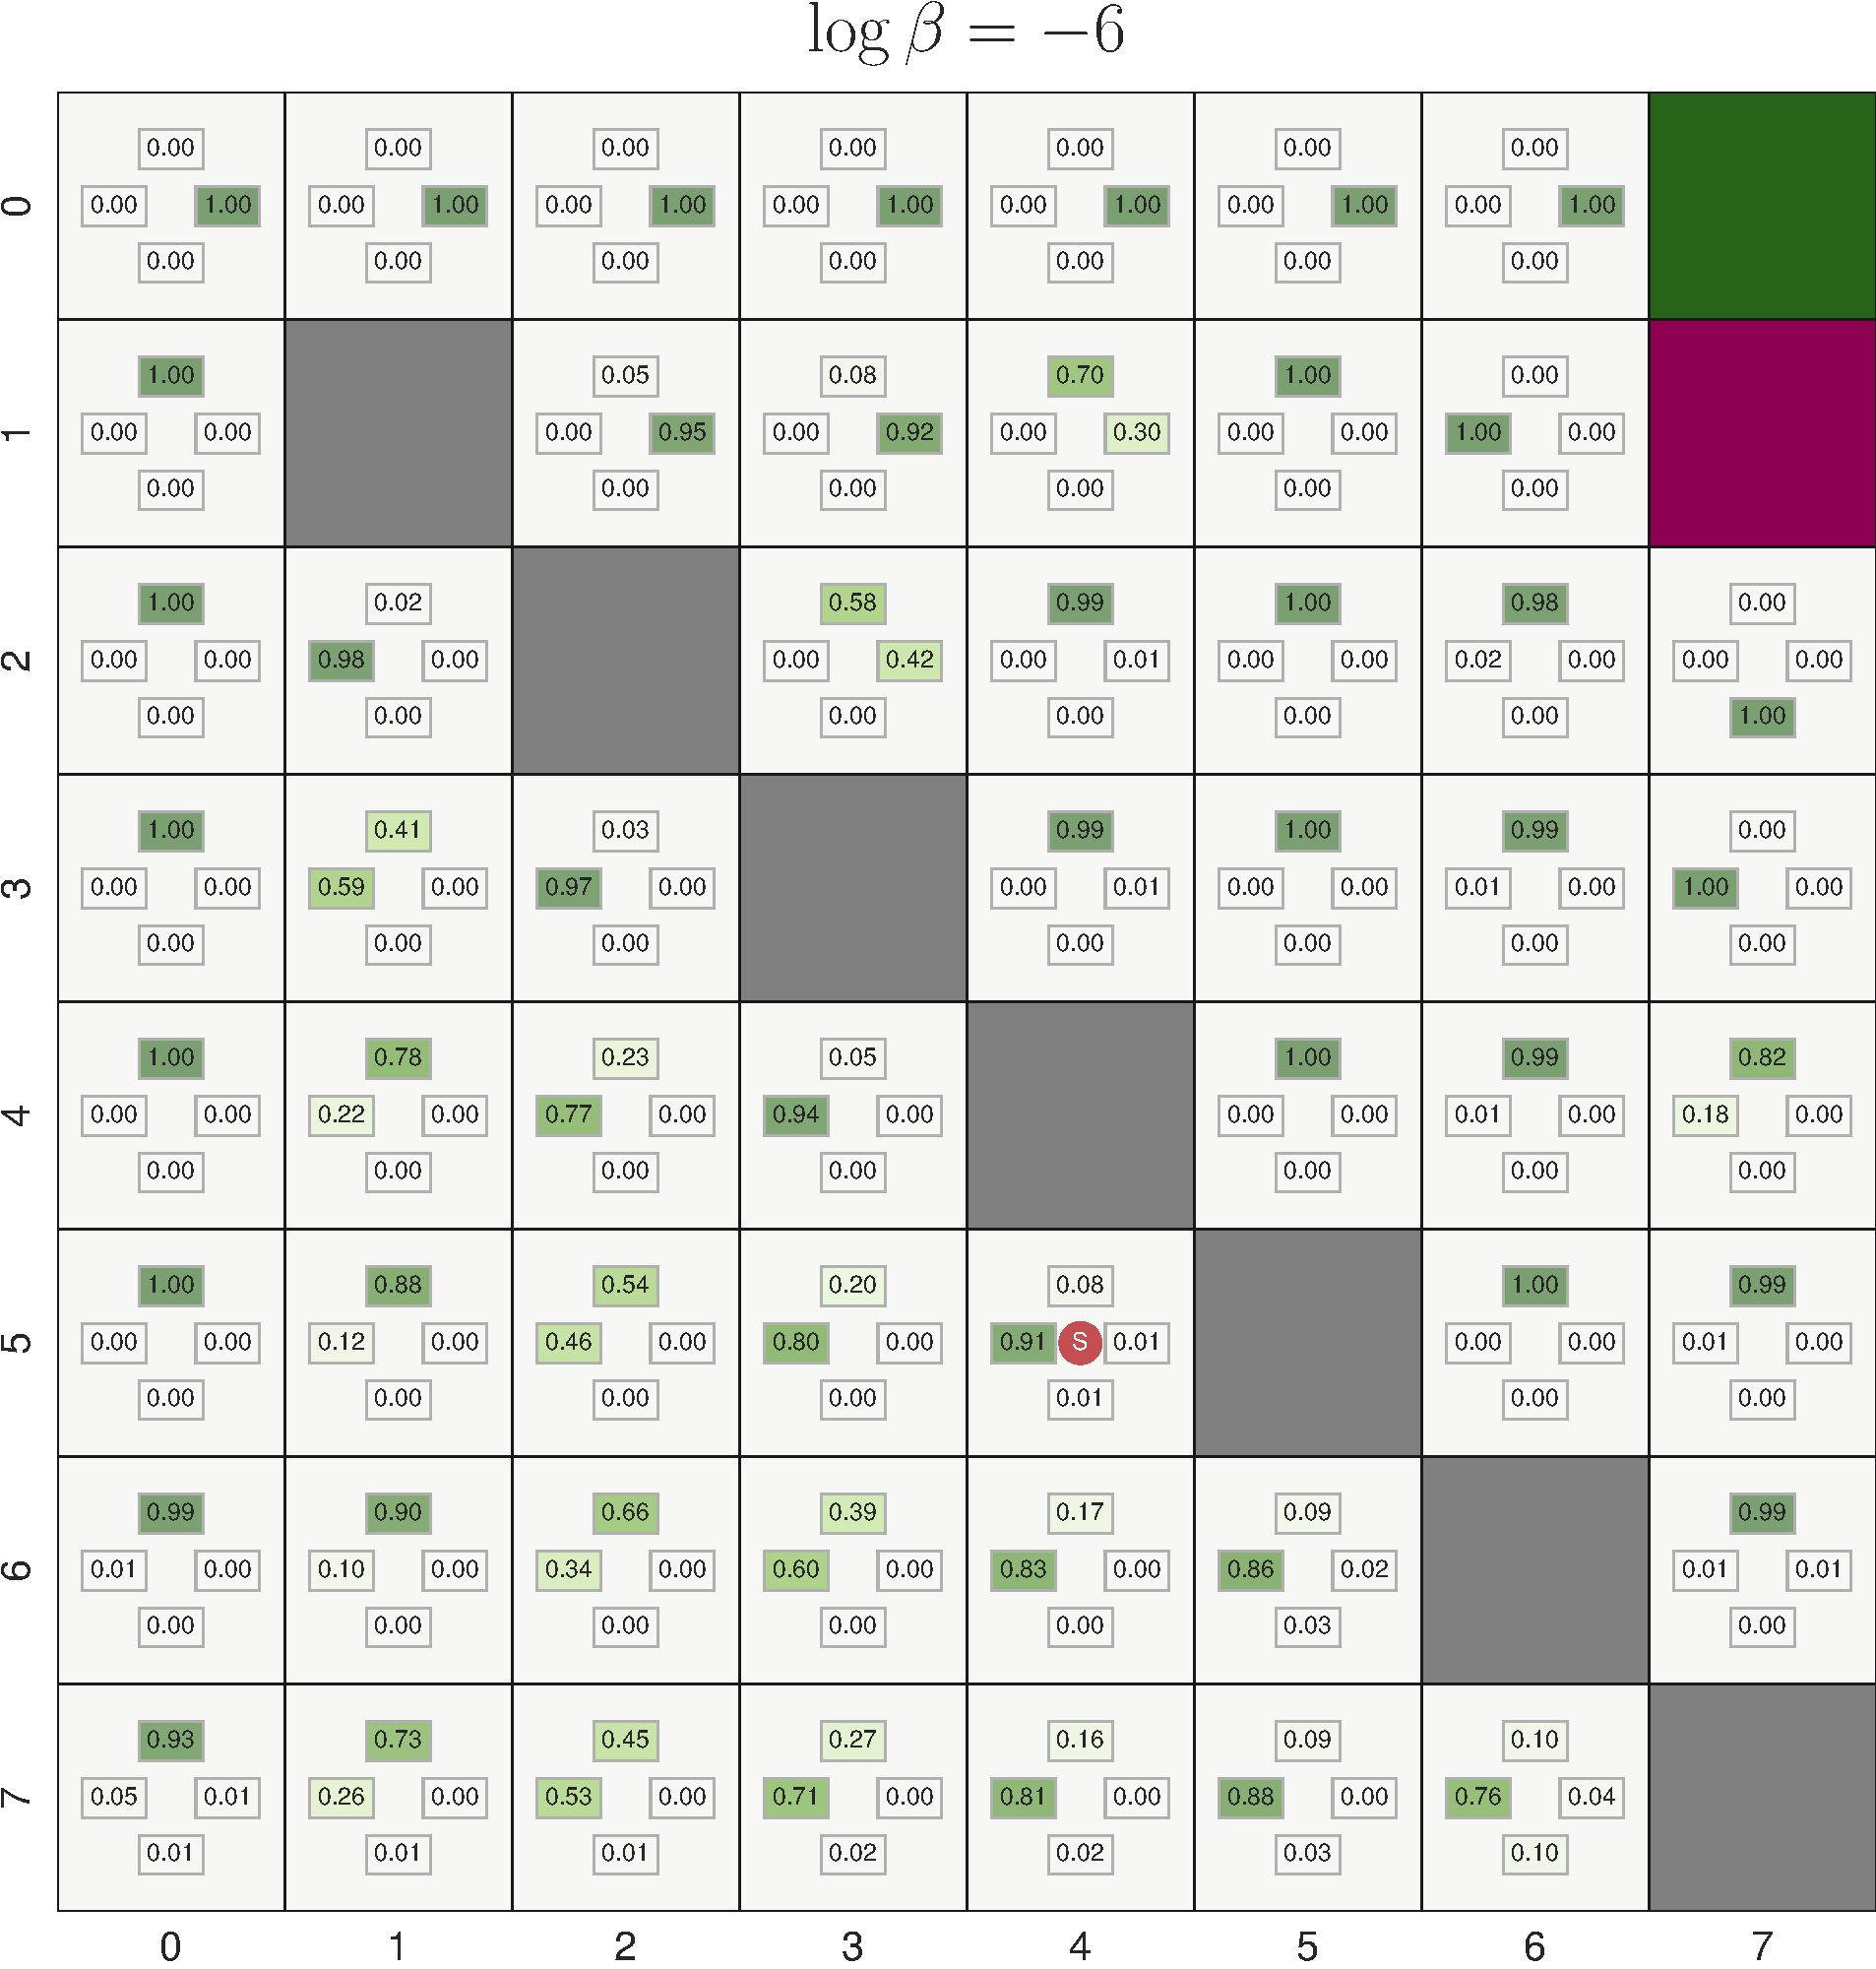
\includegraphics[width=\linewidth]{figs/ch3/gw_beta-6.pdf}
    \end{minipage}
    \hfill
    \begin{minipage}[b]{0.48\linewidth}
        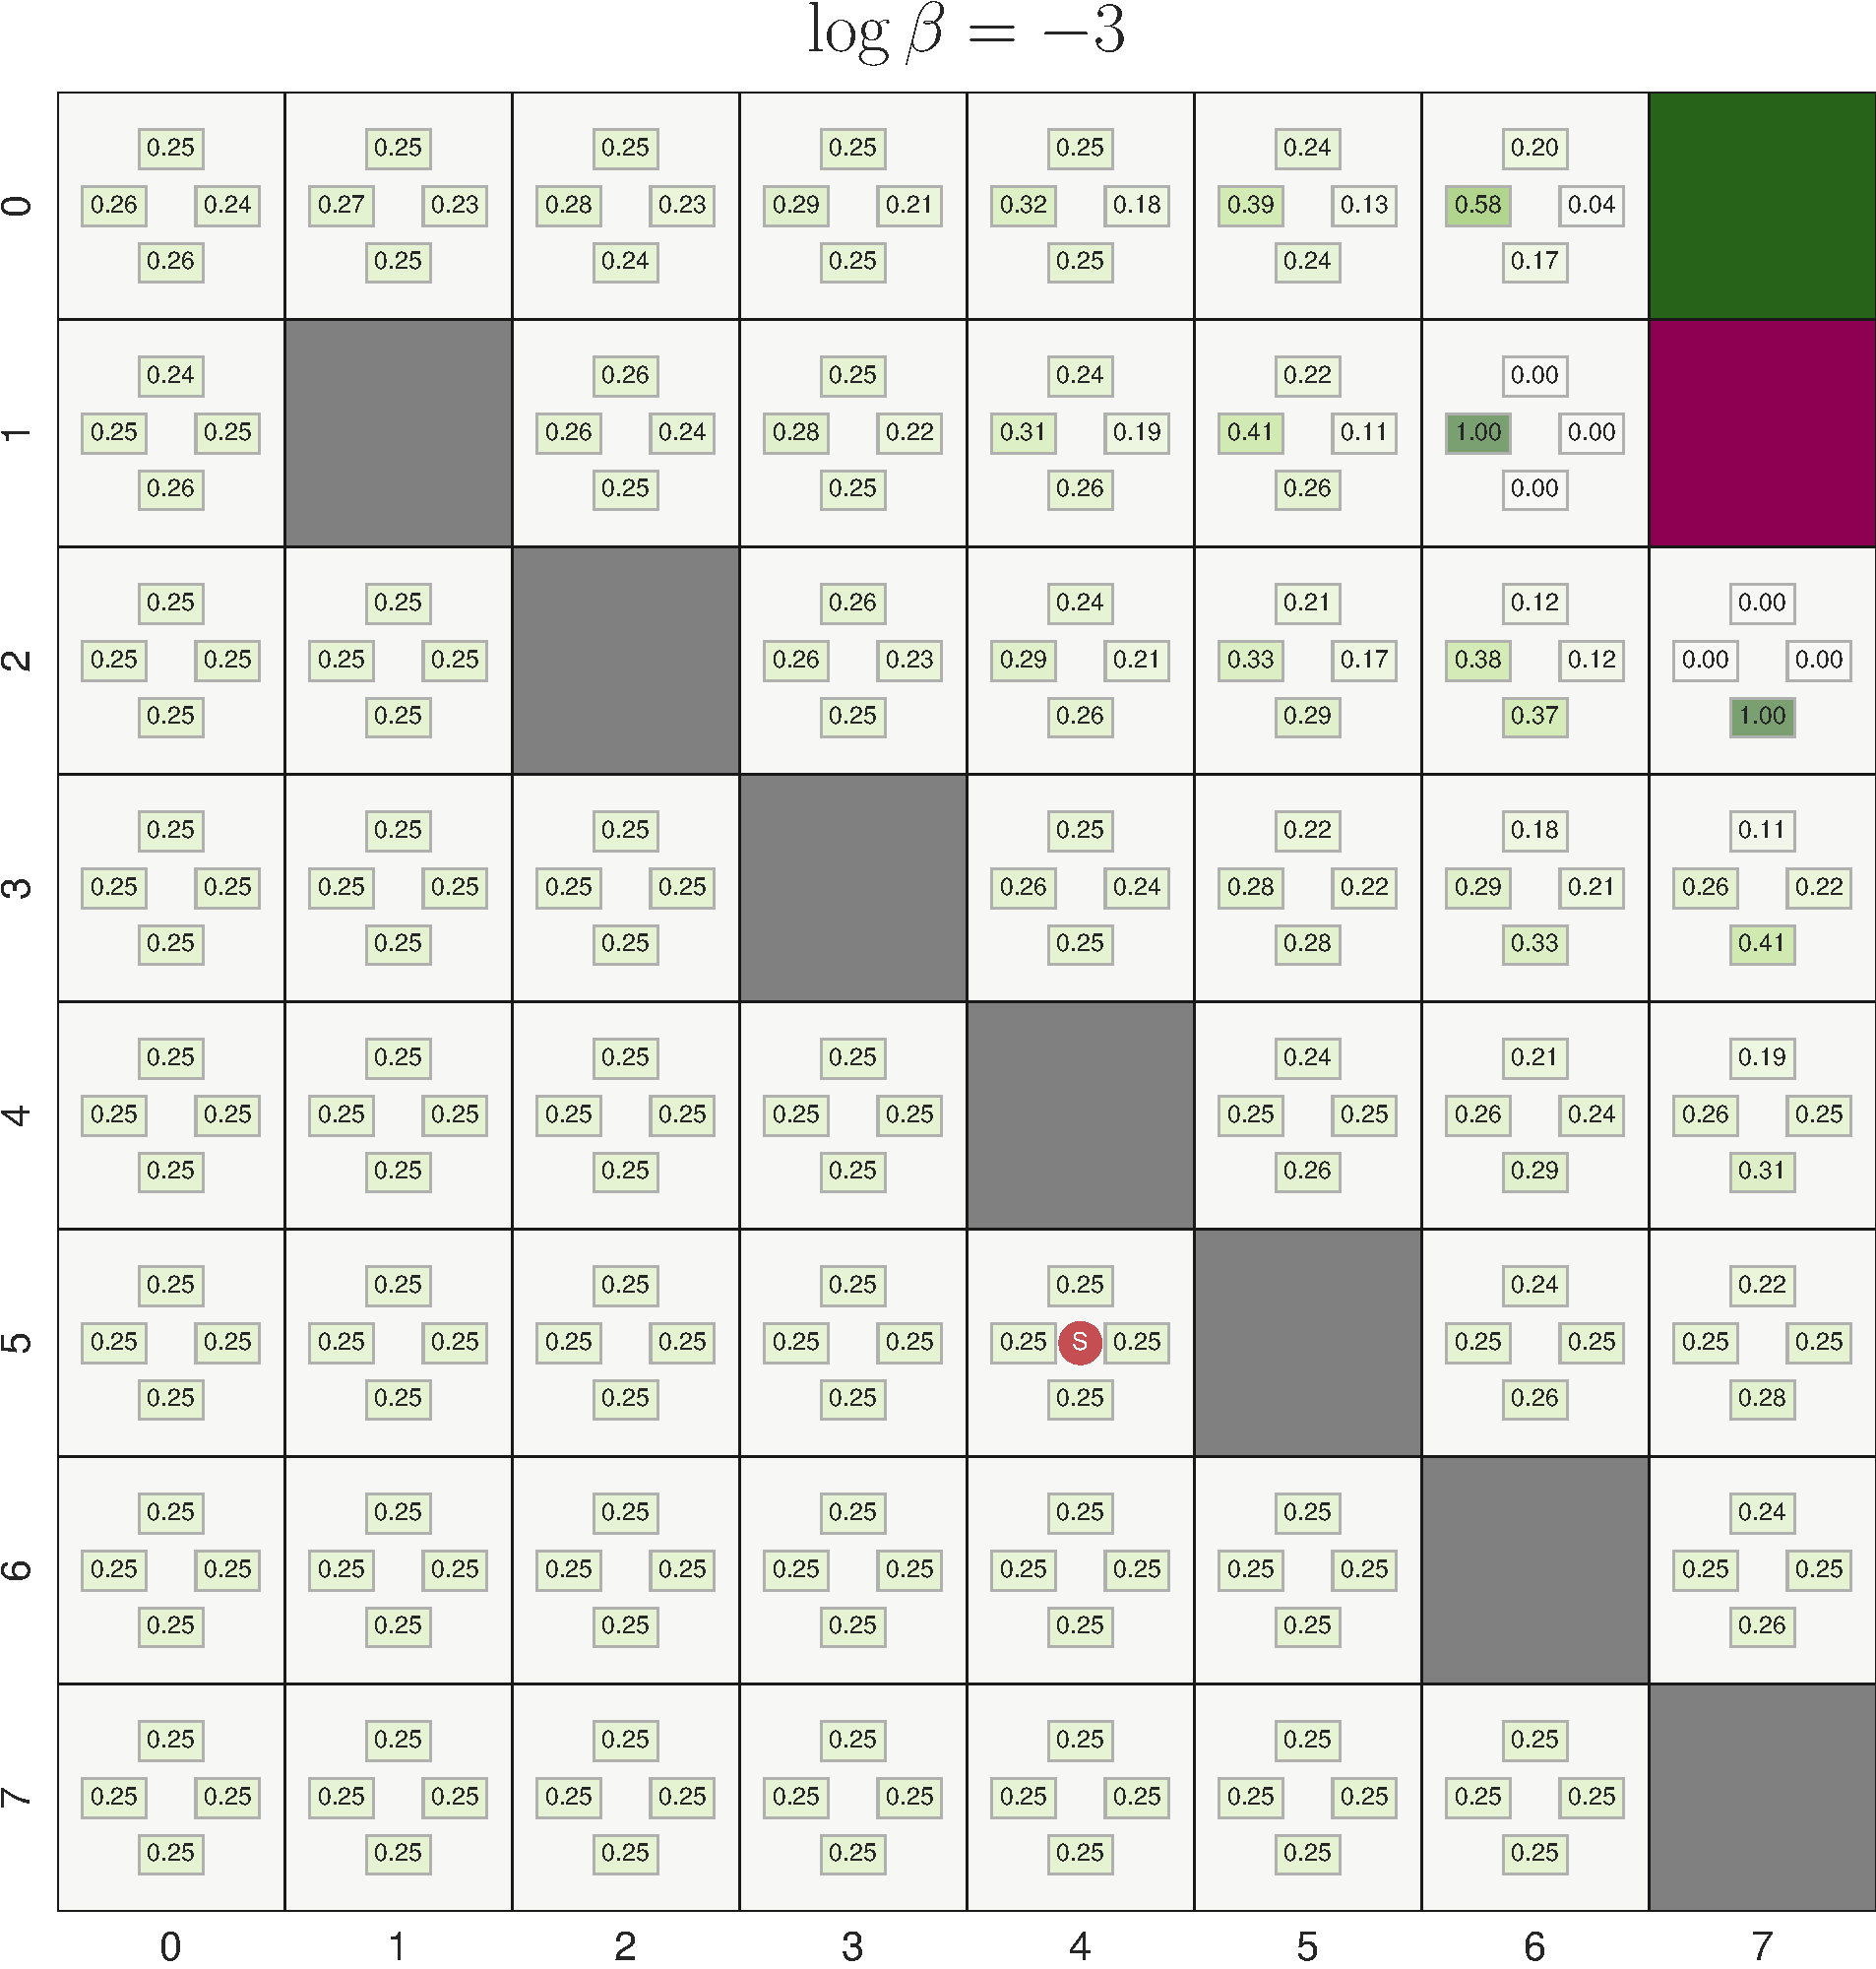
\includegraphics[width=\linewidth]{figs/ch3/gw_beta-3.pdf}
    \end{minipage}
    \vspace{5pt}
    \caption{The Maximum Entropy policy learned through Soft Q-Value iteration of Algorithm~\ref{ch3:alg:softq}, for $\log\beta=-6$ (left) and $\log\beta=-3$ (right).}\label{ch3:fig:twobetas}
    % \vspace{-1em}
\end{figure}
\FloatBarrier

We compare our proposed compression algorithm in Algorithm~\ref{ch3:alg:search} with a baseline of uniform quantization. As detailed in Algorithm~\ref{ch3:alg:uniformquant}, given an entropy budget $R$, the input symbols are uniformly partitioned into $\lfloor 2^R \rfloor$ groups, and each group is encoded into the same code.

\begin{algorithm}
\caption{Uniform Quantizer Encoder}\label{ch3:alg:uniformquant}
\begin{algorithmic}[1] 
    \Require $p_X, R$
    \Ensure $p_{XT}$

    \State $n \gets \text{length of } p_X$
    \State $m \gets \lfloor 2^R \rfloor$ 
    \State $\text{partition\_size} \gets \lceil n / m \rceil$
    \State Initialize $p_{XT}$ as an $n \times m$ zero matrix
    \For{$i \gets 0$ \textbf{to} $m-1$}           % The \For{} loop
        \State $start \gets i \times \text{partition\_size}$
        \State $end \gets \min(start + \text{partition\_size}, n)$
        \State $p_{XT}[start:end, i] \gets p_X[start:end]$
    \EndFor
    \State\Return $p_{XT}$      
\end{algorithmic}
\end{algorithm}

Figure~\ref{ch3:fig:tradeoff} illustrates the trade-off between MDP reward and the receiver's accuracy for different values of \(\beta\), using our deterministic mapping search algorithm for EBIM in Algorithm~\ref{ch3:alg:search} and the uniform quantization encoder in Algorithm~\ref{ch3:alg:uniformquant}. Here, the compression rate is defined by the ratio of the entropy of the message to the allowed code budget \(H(T)\).

\begin{figure}
    \centering
    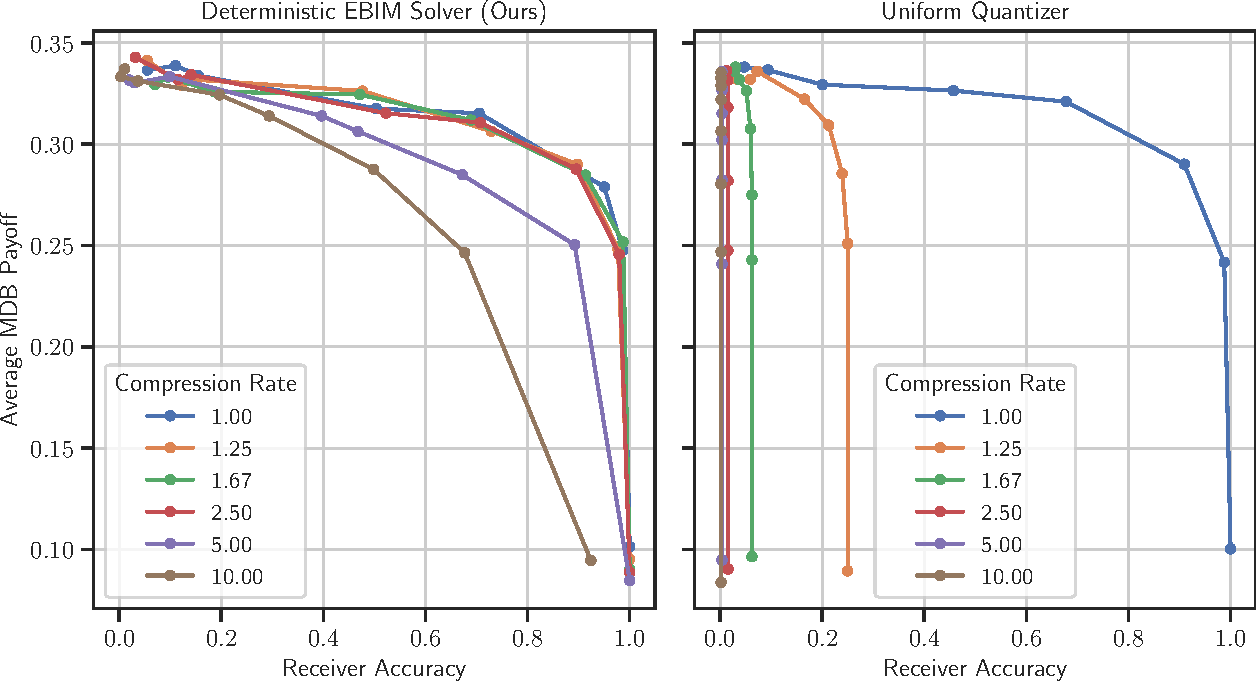
\includegraphics[width=\linewidth]{figs/ch3/tradeoff.pdf}
    \caption{
    The trade-off between the MDP reward vs. receiver's accuracy navigated for different values of $\beta$. Left: using our search algorithm for compression (Algorithm~\ref{ch3:alg:search}), Right: using uniform quantization in Algorithm~\ref{ch3:alg:uniformquant}.
    }
    \label{ch3:fig:tradeoff}
\end{figure}

\begin{figure}
    \centering
    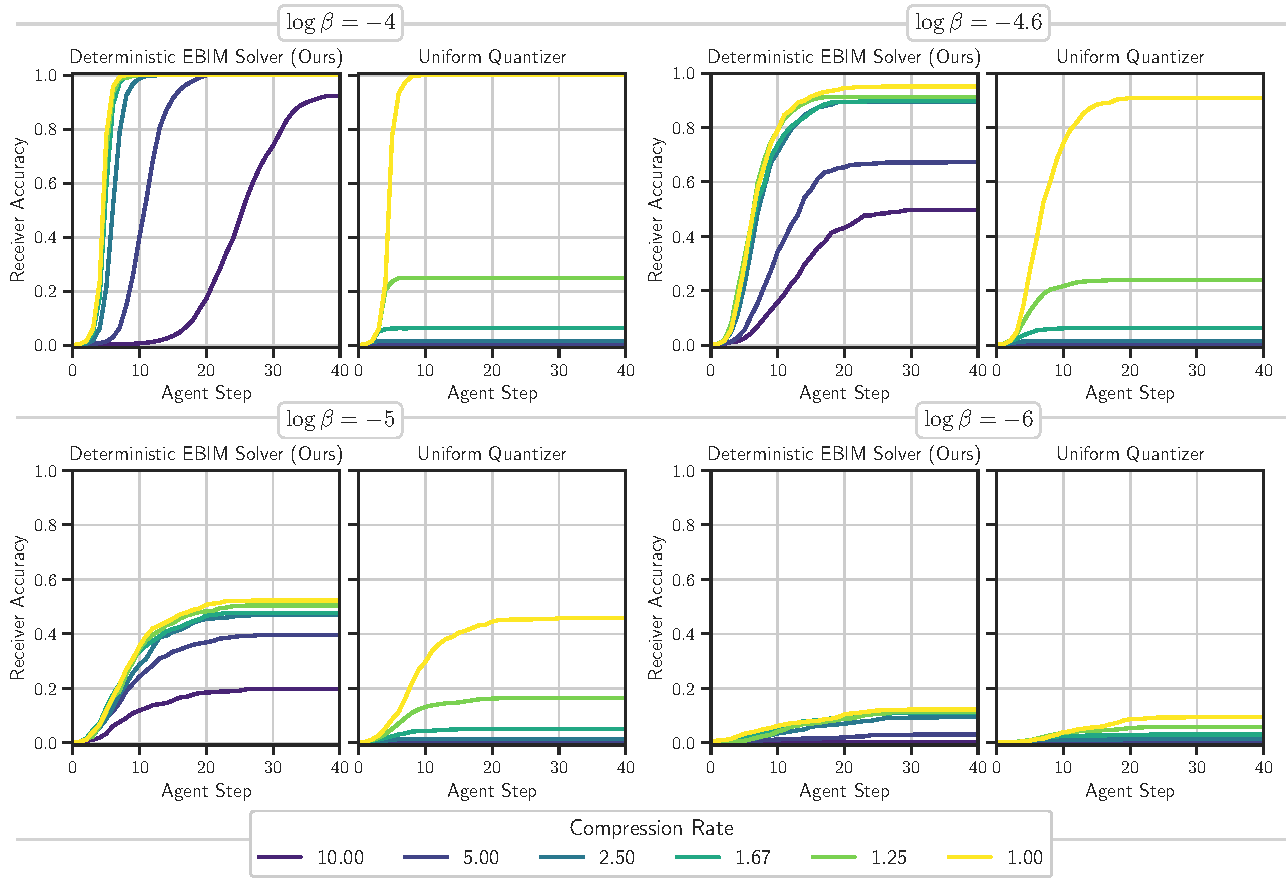
\includegraphics[width=\textwidth]{figs/ch3/accvssteps3.pdf}
    \vspace{1pt}
    % \caption{Evolution of message belief over time, for various values of $\beta$ (rows) and rate budget (colors), using our search algorithm for compression in Algorithm~\ref{ch3:alg:search} (left column) vs. uniform quantization in Algorithm~\ref{ch3:alg:uniformquant} (right column).}
    \caption{Evolution of message belief over time, for various values of $\beta$ and rate budget, using our search algorithm for compression in Algorithm~\ref{ch3:alg:search} vs. uniform quantization in Algorithm~\ref{ch3:alg:uniformquant}.}
    
    \label{ch3:fig:accvssteps}
\end{figure}

Figure~\ref{ch3:fig:accvssteps} illustrates the evolution of message belief over time for various values of \(\beta\) and rate budgets. A marginal policy optimized with a higher \(\beta\) prioritizes message accuracy over MDP payoff, as higher entropy of actions at each state provides more room for the agent to encode information about the message. Consequently, as observed, this leads to improved receiver accuracy in fewer steps. In addition, a lower compression rate permits the agent to retain more information about the message, enabling more effective encoding of information in the selected trajectory.


% \clearpage
\FloatBarrier

\section{Summary and Concluding Remarks}

We investigated a lossy compression framework under logarithmic loss, where the output distribution differs from the source distribution. This framework supports joint compression and retrieval applications such as super-resolution from compressed data, or more generally, cases where distributional shifts occur due to processing. We demonstrated that this framework effectively extends the classical minimum entropy coupling by incorporating a bottleneck, which regulates the degree of stochasticity or determinism in the coupling.

We demonstrated that separately optimizing the encoder and decoder decomposes the Minimum Entropy Coupling with Bottleneck (MEC-B) into two distinct problems: Entropy-Bounded Information Maximization (EBIM) for the encoder, followed by Minimum Entropy Coupling (MEC) for the decoder. We conducted an extensive study of the EBIM problem, provided a functional mapping search algorithm with guaranteed performance, and characterized the optimal solution adjacent to functional mappings, offering valuable theoretical insights into the problem structure.

To illustrate an application of MEC-B, the chapter presented experiments on Markov Coding Games (MCGs) with rate limits. MCGs involve a sender, an agent, and a receiver, where the agent aims to convey a message from the sender to the receiver through actions within a Markov Decision Process (MDP). The chapter focused on a rate-limited MCG where the agent receives a compressed version of the message iteratively and encodes information about the message into the MDP trajectory for the receiver. Experiments were conducted using GridWorld environment as the MDP. The results demonstrated the trade-off between MDP reward and receiver accuracy, with varying compression rates, compared to baseline compression schemes.

% future directions
% Future research could focus on quantifying the gap between the separate optimization of the encoder and decoder and the optimal joint setting.
% Understanding this gap can lead to the development of methods that jointly optimize both components, potentially improving the current solution.

% Also, as evident in Figure~\ref{ch3:fig:tradeoff}, the current solution controls the entropy of the coupling by mapping parts of input to output deterministically, while leaving others completely stochastic. Enabling fine-grained control over the entropy is spread in the coupling can be key in some applications. Additionally, the application of Entropy-Bounded Information Maximization (EBIM) in watermarking language models \cite{kirchenbauer2023watermark} suggests a valuable intersection with state-of-the-art AI applications.

% Moreover, extending this framework to continuous cases could lead to the design of neural network architectures based on the proposed model and provide information-theoretic insights into a broad spectrum of deep learning problems. These include unpaired sample-to-sample translation \cite{isola2016image, zhu2017unpaired, hoffman2018cycada}, joint compression and upscaling \cite{kang2019toward, liu2021lossy}, and the InfoMax framework \cite{tschannen2019mutual, hjelm2018learning}, among others.

% A significant challenge in the continuous case is the issue of distribution permutations: within the current framework, solutions can be achieved by maximizing the mutual information between bijective functions of input and output. A straightforward example of this is swapping the channels of images in the input and output while still maintaining maximal mutual information. Proposing strategies to mitigate this issue is another potential direction for future research in the continuous domain.


